%        File: arfc-beamer.tex
%     Created: Sun May 5 10:00 PM 2013 C
%


%\documentclass[11pt,handout]{beamer}
\documentclass[9pt]{beamer}
\usetheme[white]{Illinois}
\title[Short Title]{Demand Driven Deployment Capabilities in \Cyclus}
\author[Your Name]{Gwendolyn J. Chee$^1$, Roberto E. Fairhurst Agosta$^1$, Jin Whan Bae$^2$, Robert R. Flanagan$^3$, and Kathryn D. Huff$^1$}
\date[09.24.2019]{September 24, 2019}
\institute{
$^1$Dept. of Nuclear, Plasma and Radiological Engineering, University of Illinois at Urbana-Champaign \\
$^2$ Oak Ridge National Laboratory, Oak Ridge, TN, United States \\
$^3$Nuclear Engineering Program, University of South Carolina \\
}

%\usepackage{bbding}
\usepackage{amsfonts}
\usepackage{amsmath}
\usepackage{xspace}
\usepackage{graphicx}
\usepackage{booktabs} % nice rules for tables
\usepackage{microtype} % if using PDF
\usepackage{bigints}
\usepackage{minted}
\usepackage{subfigure}

\newcommand{\Cyclus}{\textsc{Cyclus}\xspace}%
\newcommand{\Cycamore}{\textsc{Cycamore}\xspace}%
\newcommand{\deploy}{\texttt{d3ploy}\xspace}%
\newcommand{\units}[1] {\:\text{#1}}%
\newcommand{\SN}{S$_N$}%{S$_\text{N}$}%{$S_N$}%
\DeclareMathOperator{\erf}{erf}
%I need some complimentary error funcitons... 
\DeclareMathOperator{\erfc}{erfc}
%page numbers
\setbeamertemplate{footline}[page number]
\setbeamertemplate{caption}[numbered]
%Those icons in the references are terrible looking
\setbeamertemplate{bibliography item}[text]

\usepackage{tikz}
\usetikzlibrary{positioning, arrows, decorations, shapes}

\usetikzlibrary{shapes.geometric,arrows}
\tikzstyle{process} = [rectangle, rounded corners, minimum width=3cm, minimum height=1cm,text centered, draw=black, fill=blue!30]
\tikzstyle{object} = [ellipse, rounded corners, minimum width=3cm, minimum height=1cm,text centered, draw=black, fill=green!30]
\tikzstyle{arrow} = [thick,->,>=stealth]

\definecolor{illiniblue}{HTML}{B1C6E2}
\definecolor{illiniorange}{HTML}{f8c2a2}
\usetikzlibrary{shapes.geometric, arrows}
\tikzstyle{oblock} = [rectangle, draw, fill=illiniorange, 
text width=15em, text centered, rounded corners, minimum height=4em]
\tikzstyle{bblock} = [rectangle, draw, fill=illiniblue, 
text width=15em, text centered, rounded corners, minimum height=4em]
\tikzstyle{arrow} = [thick,->,>=stealth]

\usepackage{tabularx}
\newcolumntype{b}{>{\hsize=1.0\hsize}X}
\newcolumntype{s}{>{\hsize=.5\hsize}X}
\newcolumntype{m}{>{\hsize=.75\hsize}X}
\newcolumntype{x}{>{\hsize=.25\hsize}X}
\newcolumntype{L}{>{\raggedright\arraybackslash}X}
\newcolumntype{R}{>{\raggedleft\arraybackslash}X}
\def\arraystretch{1}
%%%% Acronym support
\usepackage{multirow}
\usepackage{graphicx,subfigure}

\usepackage[acronym,toc]{glossaries}
%\newacronym{<++>}{<++>}{<++>}
\newacronym[longplural={metric tons of heavy metal}]{MTHM}{MTHM}{metric ton of heavy metal}
\newacronym{ABM}{ABM}{agent-based modeling}
\newacronym{ACDIS}{ACDIS}{Program in Arms Control \& Domestic and International Security}
\newacronym{AHTR}{AHTR}{Advanced High Temperature Reactor}
\newacronym{ANDRA}{ANDRA}{Agence Nationale pour la gestion des D\'echets RAdioactifs, the French National Agency for Radioactive Waste Management}
\newacronym{ANL}{ANL}{Argonne National Laboratory}
\newacronym{API}{API}{application programming interface}
\newacronym{ARE}{ARE}{Aircraft Reactor Experiment}
\newacronym{ARFC}{ARFC}{Advanced Reactors and Fuel Cycles}
\newacronym{ASME}{ASME}{American Society of Mechanical Engineers}
\newacronym{ATWS}{ATWS}{Anticipated Transient Without Scram}
\newacronym{BDBE}{BDBE}{Beyond Design Basis Event}
\newacronym{BIDS}{BIDS}{Berkeley Institute for Data Science}
\newacronym{CAFCA}{CAFCA}{ Code for Advanced Fuel Cycles Assessment }
\newacronym{CDTN}{CDTN}{Centro de Desenvolvimento da Tecnologia Nuclear}
\newacronym{CEA}{CEA}{Commissariat \`a l'\'Energie Atomique et aux \'Energies Alternatives}
\newacronym{CI}{CI}{continuous integration}
\newacronym{CNEN}{CNEN}{Comiss\~{a}o Nacional de Energia Nuclear}
\newacronym{CNERG}{CNERG}{Computational Nuclear Engineering Research Group}
\newacronym{COSI}{COSI}{Commelini-Sicard}
\newacronym{COTS}{COTS}{commercial, off-the-shelf}
\newacronym{CSNF}{CSNF}{commercial spent nuclear fuel}
\newacronym{CTAH}{CTAHs}{Coiled Tube Air Heaters}
\newacronym{CUBIT}{CUBIT}{CUBIT Geometry and Mesh Generation Toolkit}
\newacronym{CURIE}{CURIE}{Centralized Used Fuel Resource for Information Exchange}
\newacronym{DAG}{DAG}{directed acyclic graph}
\newacronym{DANESS}{DANESS}{Dynamic Analysis of Nuclear Energy System Strategies}
\newacronym{DBE}{DBE}{Design Basis Event}
\newacronym{DESAE}{DESAE}{Dynamic Analysis of Nuclear Energy Systems Strategies}
\newacronym{DHS}{DHS}{Department of Homeland Security}
\newacronym{DOE}{DOE}{Department of Energy}
\newacronym{DRACS}{DRACS}{Direct Reactor Auxiliary Cooling System}
\newacronym{DRE}{DRE}{dynamic resource exchange}
\newacronym{DSNF}{DSNF}{DOE spent nuclear fuel}
\newacronym{DYMOND}{DYMOND}{Dynamic Model of Nuclear Development }
\newacronym{EBS}{EBS}{Engineered Barrier System}
\newacronym{EDZ}{EDZ}{Excavation Disturbed Zone}
\newacronym{EIA}{EIA}{U.S. Energy Information Administration}
\newacronym{EPA}{EPA}{Environmental Protection Agency}
\newacronym{EP}{EP}{Engineering Physics}
\newacronym{FCO}{FCO}{Fuel Cycle Options}
\newacronym{FCT}{FCT}{Fuel Cycle Technology}
\newacronym{FEHM}{FEHM}{Finite Element Heat and Mass Transfer}
\newacronym{FEPs}{FEPs}{Features, Events, and Processes}
\newacronym{FHR}{FHR}{Fluoride-Salt-Cooled High-Temperature Reactor}
\newacronym{FLiBe}{FLiBe}{Fluoride-Lithium-Beryllium}
\newacronym{GDSE}{GDSE}{Generic Disposal System Environment}
\newacronym{GDSM}{GDSM}{Generic Disposal System Model}
\newacronym{GENIUSv1}{GENIUSv1}{Global Evaluation of Nuclear Infrastructure Utilization Scenarios, Version 1}
\newacronym{GENIUSv2}{GENIUSv2}{Global Evaluation of Nuclear Infrastructure Utilization Scenarios, Version 2}
\newacronym{GENIUS}{GENIUS}{Global Evaluation of Nuclear Infrastructure Utilization Scenarios}
\newacronym{GPAM}{GPAM}{Generic Performance Assessment Model}
\newacronym{GRSAC}{GRSAC}{Graphite Reactor Severe Accident Code}
\newacronym{GUI}{GUI}{graphical user interface}
\newacronym{HLW}{HLW}{high level waste}
\newacronym{HPC}{HPC}{high-performance computing}
\newacronym{HTC}{HTC}{high-throughput computing}
\newacronym{HTGR}{HTGR}{High Temperature Gas-Cooled Reactor}
\newacronym{IAEA}{IAEA}{International Atomic Energy Agency}
\newacronym{IEMA}{IEMA}{Illinois Emergency Mangament Agency}
\newacronym{INL}{INL}{Idaho National Laboratory}
\newacronym{IPRR1}{IRP-R1}{Instituto de Pesquisas Radioativas Reator 1}
\newacronym{IRP}{IRP}{Integrated Research Project}
\newacronym{ISFSI}{ISFSI}{Independent Spent Fuel Storage Installation}
\newacronym{ISRG}{ISRG}{Independent Student Research Group}
\newacronym{JFNK}{JFNK}{Jacobian-Free Newton Krylov}
\newacronym{LANL}{LANL}{Los Alamos National Laboratory}
\newacronym{LBNL}{LBNL}{Lawrence Berkeley National Laboratory}
\newacronym{LCOE}{LCOE}{levelized cost of electricity}
\newacronym{LDRD}{LDRD}{laboratory directed research and development}
\newacronym{LFR}{LFR}{Lead-Cooled Fast Reactor}
\newacronym{LLNL}{LLNL}{Lawrence Livermore National Laboratory}
\newacronym{LMFBR}{LMFBR}{Liquid Metal Fast Breeder Reactor}
\newacronym{LOFC}{LOFC}{Loss of Forced Cooling}
\newacronym{LOHS}{LOHS}{Loss of Heat Sink}
\newacronym{LOLA}{LOLA}{Loss of Large Area}
\newacronym{LP}{LP}{linear program}
\newacronym{LWR}{LWR}{Light Water Reactor}
\newacronym{MA}{MA}{minor actinide}
\newacronym{MCNP}{MCNP}{Monte Carlo N-Particle code}
\newacronym{MILP}{MILP}{mixed-integer linear program}
\newacronym{MIT}{MIT}{the Massachusetts Institute of Technology}
\newacronym{MOAB}{MOAB}{Mesh-Oriented datABase}
\newacronym{MOOSE}{MOOSE}{Multiphysics Object-Oriented Simulation Environment}
\newacronym{MOX}{MOX}{mixed oxide}
\newacronym{MSBR}{MSBR}{Molten Salt Breeder Reactor}
\newacronym{MSRE}{MSRE}{Molten Salt Reactor Experiment}
\newacronym{MSR}{MSR}{Molten Salt Reactor}
\newacronym{NAGRA}{NAGRA}{National Cooperative for the Disposal of Radioactive Waste}
\newacronym{NEAMS}{NEAMS}{Nuclear Engineering Advanced Modeling and Simulation}
\newacronym{NEUP}{NEUP}{Nuclear Energy University Programs}
\newacronym{NFCSim}{NFCSim}{Nuclear Fuel Cycle Simulator}
\newacronym{NGNP}{NGNP}{Next Generation Nuclear Plant}
\newacronym{NMWPC}{NMWPC}{Nuclear MW Per Capita}
\newacronym{NNSA}{NNSA}{National Nuclear Security Administration}
\newacronym{NPRE}{NPRE}{Department of Nuclear, Plasma, and Radiological Engineering}
\newacronym{NQA1}{NQA-1}{Nuclear Quality Assurance - 1}
\newacronym{NRC}{NRC}{Nuclear Regulatory Commission}
\newacronym{NSF}{NSF}{National Science Foundation}
\newacronym{NSSC}{NSSC}{Nuclear Science and Security Consortium}
\newacronym{NUWASTE}{NUWASTE}{Nuclear Waste Assessment System for Technical Evaluation}
\newacronym{NWF}{NWF}{Nuclear Waste Fund}
\newacronym{NWTRB}{NWTRB}{Nuclear Waste Technical Review Board}
\newacronym{OCRWM}{OCRWM}{Office of Civilian Radioactive Waste Management}
\newacronym{ORION}{ORION}{ORION}
\newacronym{ORNL}{ORNL}{Oak Ridge National Laboratory}
\newacronym{PARCS}{PARCS}{Purdue Advanced Reactor Core Simulator}
\newacronym{PBAHTR}{PB-AHTR}{Pebble Bed Advanced High Temperature Reactor}
\newacronym{PBFHR}{PB-FHR}{Pebble-Bed Fluoride-Salt-Cooled High-Temperature Reactor}
\newacronym{PEI}{PEI}{Peak Environmental Impact}
\newacronym{PH}{PRONGHORN}{PRONGHORN}
\newacronym{PRKE}{PRKE}{Point Reactor Kinetics Equations}
\newacronym{PSPG}{PSPG}{Pressure-Stabilizing/Petrov-Galerkin}
\newacronym{PWAR}{PWAR}{Pratt and Whitney Aircraft Reactor}
\newacronym{PWR}{PWR}{Pressurized Water Reactor}
\newacronym{PyNE}{PyNE}{Python toolkit for Nuclear Engineering}
\newacronym{PyRK}{PyRK}{Python for Reactor Kinetics}
\newacronym{QA}{QA}{quality assurance}
\newacronym{RDD}{RD\&D}{Research Development and Demonstration}
\newacronym{RD}{R\&D}{Research and Development}
\newacronym{RELAP}{RELAP}{Reactor Excursion and Leak Analysis Program}
\newacronym{RIA}{RIA}{Reactivity Insertion Accident}
\newacronym{RIF}{RIF}{Region-Institution-Facility}
\newacronym{SFR}{SFR}{Sodium-Cooled Fast Reactor}
\newacronym{SINDAG}{SINDA{\textbackslash}G}{Systems Improved Numerical Differencing Analyzer $\backslash$ Gaski}
\newacronym{SKB}{SKB}{Svensk K\"{a}rnbr\"{a}nslehantering AB}
\newacronym{SNF}{SNF}{spent nuclear fuel}
\newacronym{SNL}{SNL}{Sandia National Laboratory}
\newacronym{STC}{STC}{specific temperature change}
\newacronym{SUPG}{SUPG}{Streamline-Upwind/Petrov-Galerkin}
\newacronym{SWF}{SWF}{Separations and Waste Forms}
\newacronym{SWU}{SWU}{Separative Work Unit}
\newacronym{TRIGA}{TRIGA}{Training Research Isotope General Atomic}
\newacronym{TRISO}{TRISO}{Tristructural Isotropic}
\newacronym{TSM}{TSM}{Total System Model}
\newacronym{TSPA}{TSPA}{Total System Performance Assessment for the Yucca Mountain License Application}
\newacronym{ThOX}{ThOX}{thorium oxide}
\newacronym{UFD}{UFD}{Used Fuel Disposition}
\newacronym{UML}{UML}{Unified Modeling Language}
\newacronym{UOX}{UOX}{uranium oxide}
\newacronym{UQ}{UQ}{uncertainty quantification}
\newacronym{US}{US}{United States}
\newacronym{UW}{UW}{University of Wisconsin}
\newacronym{VISION}{VISION}{the Verifiable Fuel Cycle Simulation Model}
\newacronym{VV}{V\&V}{verification and validation}
\newacronym{WIPP}{WIPP}{Waste Isolation Pilot Plant}
\newacronym{YMR}{YMR}{Yucca Mountain Repository Site}


\makeglossaries

%try to get rid of header on title page\dots
\makeatletter
    \newenvironment{withoutheadline}{
        \setbeamertemplate{headline}[default]
        \def\beamer@entrycode{\vspace*{-\headheight}}
    }{}
\makeatother

% add slide numbers
\makeatother
\setbeamertemplate{footline}
{
  \leavevmode%
  \hbox{%
    \rightline{\insertframenumber{} / \inserttotalframenumber\hspace*{1ex}}
  }%
  \vskip0pt%
}
\makeatletter

\begin{document}
%%%%%%%%%%%%%%%%%%%%%%%%%%%%%%%%%%%%%%%%%%%%%%%%%%%%%%%%%%%%%
%% From uw-beamer Here's a handy bit of code to place at 
%% the beginning of your presentation (after \begin{document}):
\newcommand*{\alphabet}{ABCDEFGHIJKLMNOPQRSTUVWXYZabcdefghijklmnopqrstuvwxyz}
\newlength{\highlightheight}
\newlength{\highlightdepth}
\newlength{\highlightmargin}
\setlength{\highlightmargin}{2pt}
\settoheight{\highlightheight}{\alphabet}
\settodepth{\highlightdepth}{\alphabet}
\addtolength{\highlightheight}{\highlightmargin}
\addtolength{\highlightdepth}{\highlightmargin}
\addtolength{\highlightheight}{\highlightdepth}
\newcommand*{\Highlight}{\rlap{\textcolor{HighlightBackground}{\rule[-\highlightdepth]{\linewidth}{\highlightheight}}}}
%%%%%%%%%%%%%%%%%%%%%%%%%%%%%%%%%%%%%%%%%%%%%%%%%%%%%%%%%%%%%
%%--------------------------------%%
\begin{withoutheadline}
\frame{
  \titlepage
}
\end{withoutheadline}

%%--------------------------------%%
\AtBeginSection[]{
\begin{frame}
  \frametitle{Outline}
  \tableofcontents[currentsection]
\end{frame}
}

\section{Background and Motivation}
\subsection{Cyclus}
\begin{frame}
    \frametitle{Cyclus}
        \texttt{Cyclus} is an agent-based nuclear fuel cycle simulator with a modular architecture.
        It has three types of agents: \texttt{Facility}, \texttt{Institution}, and \texttt{Region}.
     \\   
    \begin{figure}[htbp!]
      \begin{center}
        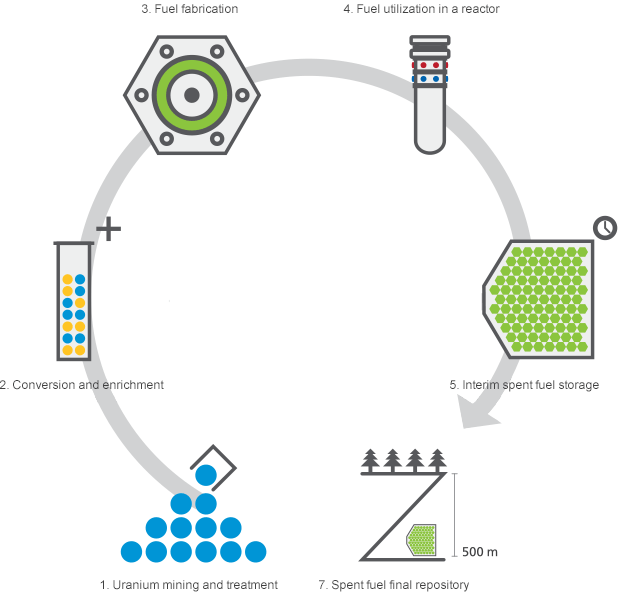
\includegraphics[height=4.5cm]{../paper/figures/nfc}
      \end{center}
            \caption{Once Through Nuclear Fuel Cycle \cite{huff_fundamental_2016}}
      \label{fig:cyclus-modular}
    \end{figure}
  \end{frame}
  
  \begin{frame}
    \frametitle{Motivation}

    \textbf{Gap in capability: User must define when support facilities are deployed.} 

    \begin{figure}[htbp!]
      \begin{center}
        
\includegraphics[width=0.8\textwidth]{../paper/figures/user-deploy}
      \end{center}
            \caption{User defined Deployment Scheme }
    \end{figure}

    \textbf{Bridging the gap: Developed \deploy, a demand-driven deployment capability in \Cyclus.}

    \begin{figure}[htbp!]
      \begin{center}
        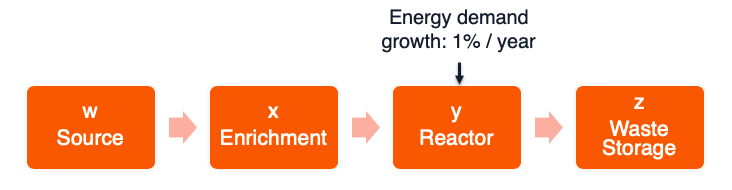
\includegraphics[width=0.8\textwidth]{../paper/figures/auto-deploy}
      \end{center}
            \caption{Demand Driven Deployment Scheme}
    \end{figure}

  \end{frame}
  
\subsection{Goal}
\begin{frame}
    \frametitle{Goals}
    \textbf{Goals of this work} 
    \begin{itemize}
        \item Develop demand driven deployment capabilities in \Cyclus (\deploy)
        \item Demonstrate the use of \deploy to set up transition scenarios 
        from the current once through \gls{LWR} fuel cycle to four other more 
        promising fuel cycles. 
    \end{itemize}

    \begin{table}[]
        \centering
        \caption{Descriptions of the current and other high performing nuclear fuel cycle evaluation groups described in the evaluation and screening study \cite{wigeland_nuclear_2014}.}
        \label{tab:eg}
            \footnotesize
            \begin{tabularx}{\textwidth}{l|lll}
                \hline
            \textbf{Fuel Cycle}                                               & \textbf{Open or Closed} & \textbf{Fuel Type}                                                              & \textbf{Reactor Type}                                                                           \\ \hline
            \textbf{\begin{tabular}[c]{@{}l@{}}EG01\\ (current)\end{tabular}} & Open                                                               & Enriched-U                                                                      & Thermal critical reactors                                                                       \\ 
            \textbf{EG23}                                                     & Closed                                                             & \begin{tabular}[c]{@{}l@{}}Recycle of U/Pu \\ with natural-U fuel\end{tabular}  & Fast critical reactors                                                                          \\ 
            \textbf{EG24}                                                     & Closed                                                             & \begin{tabular}[c]{@{}l@{}}Recycle of U/TRU \\ with natural-U fuel\end{tabular} & Fast critical reactors                                                                          \\ 
            \textbf{EG29}                                                     & Closed                                                             & \begin{tabular}[c]{@{}l@{}}Recycle of U/Pu \\ with natural-U fuel\end{tabular}  & \begin{tabular}[c]{@{}l@{}}Fast critical reactors and \\ thermal critical reactors\end{tabular} \\ 
            \textbf{EG30} & Closed                                                             & \begin{tabular}[c]{@{}l@{}}Recycle of U/TRU \\ with natural-U fuel\end{tabular} & \begin{tabular}[c]{@{}l@{}}Fast critical reactors and \\ thermal critical reactors\end{tabular} \\ \hline
        \end{tabularx}
    \end{table}

\end{frame}
%  \begin{frame}
    \frametitle{Motivation}

    \textbf{Gap in capability: User must define when support facilities are deployed.} 

    \begin{figure}[htbp!]
      \begin{center}
        
\includegraphics[width=0.8\textwidth]{../paper/figures/user-deploy}
      \end{center}
            \caption{User defined Deployment Scheme }
    \end{figure}

    \textbf{Bridging the gap: Developed \deploy, a demand-driven deployment capability in \Cyclus.}

    \begin{figure}[htbp!]
      \begin{center}
        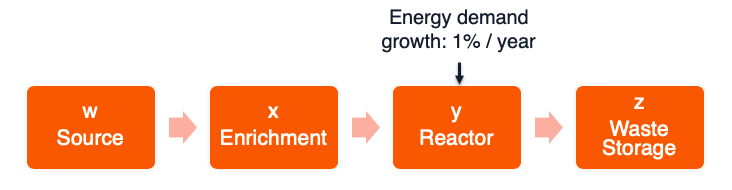
\includegraphics[width=0.8\textwidth]{../paper/figures/auto-deploy}
      \end{center}
            \caption{Demand Driven Deployment Scheme}
    \end{figure}

  \end{frame}
  

\section{Method}
\subsection{\deploy}
\begin{frame}
    \frametitle{\deploy Objectives}
    \textbf{\deploy's Main Objective}
    \vspace{0.3em}
    \\
    Minimize the number of time steps of undersupply of power.
    \vspace{1em}
    \\
    \textbf{\deploy's Sub-Objective}
    \vspace{0.3em}
    \\
    Minimize excessive oversupply of all commodities.
    \begin{align*}
    obj = min \sum_i^N |D_i-S_i|
    \end{align*}
\end{frame}

\begin{frame}
    \frametitle{\deploy Input Parameters}
    \begin{table}[]
        \centering
        \caption{\deploy's required and optional input parameters with examples.}
		\label{tab:inputs}
            \footnotesize
            {\renewcommand{\arraystretch}{1.2}
			\begin{tabularx}{\textwidth}{l|LL}
			\hline
				& \textbf{Input Parameter}                                                           & \textbf{Examples}                                                                                                          \\ \hline
				\multirow{5}{*}{\textbf{Required}} & Demand driving commodity                                                           & Power, Fuel, Plutonium, etc.                                                                                                                      \\ \hline
														  & Demand equation                                                                    & P(t) = 10000, sin(t), 10000t                                                                                                                 \\ \cline{2-3} 
														  & Available facilities                                                              & Fuel Fab, LWR reactor, Waste repository, etc.                                                                                                      \\ \cline{2-3} 
														  & Facility capacities                                                      & 3000 kg, 1000 MW, 50000 kg                                                                                                     \\ \cline{2-3} 
														  & Prediction method                                                                  & Fast Fourier Transform \\ \cline{2-3} 
														  & Deployment driving method & Installed Capacity or Supply                                                                                                               \\ \hline
				\multirow{4}{*}{\textbf{Optional}} & Buffer type                                                                        & Absolute or relative                                                                                                                 \\ \cline{2-3} 
														  & Buffer size                                                                        & \begin{tabular}[c]{@{}l@{}}Power: 3000 MW\\ Fuel: 0 kg \\ Spent fuel: 0 kg\end{tabular}                                   \\ \cline{2-3} 
														  & Facility preferences (transition time)                                                              & \begin{tabular}[c]{@{}l@{}}LWR preferred $\leq$ 100 time steps\\ SFR preferred $>$ 100 time steps \end{tabular}          \\ \cline{2-3} 
														  & Facility constraint                                                              & SFR constraint = 5000kg of Pu            \\ \hline	
						\end{tabularx}}
    \end{table}
\end{frame}

\begin{frame}
    \frametitle{\deploy logic flow}
    \begin{columns}
        \column[t]{8cm}
    \begin{figure}[]
        \centering
        \resizebox{0.8\textwidth} {0.5\height}{
        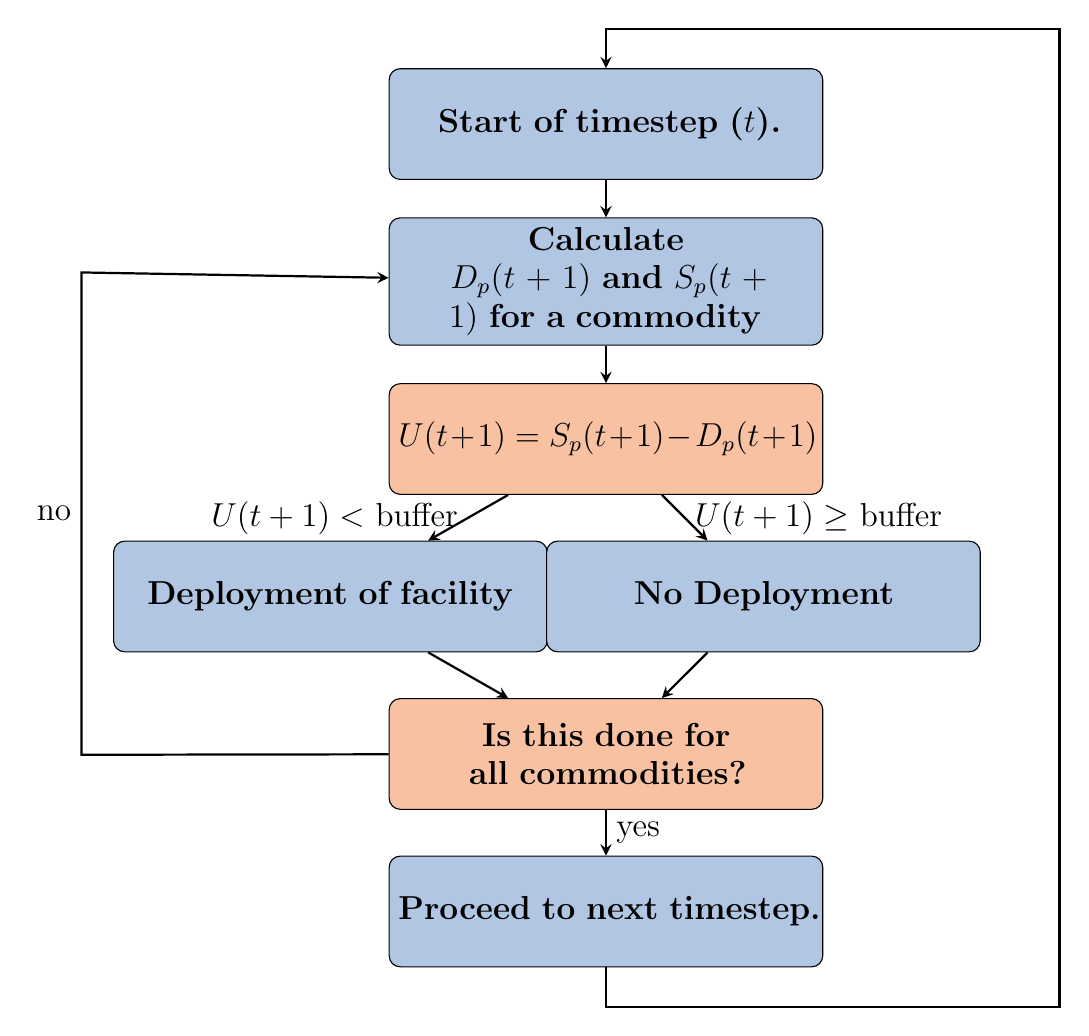
\begin{tikzpicture}[node distance=2cm]
        \tikzstyle{every node}=[font=\large]
        \node (Start) [bblock] {\textbf{Start of timestep ($t$).}};
        \node (Predict) [bblock, below of=Start] {\textbf{Calculate \\ $D_p(t+1)$ and $S_p(t+1)$ for a commodity}};
        \node (IsThere) [oblock, below of=Predict]{\textbf{$U(t+1) = S_p(t+1)-D_p(t+1)$}};
        \node (Deploy) [bblock, below of=IsThere, xshift = -3.5cm]{\textbf{Deployment of facility}};
        \node (NoDeploy) [bblock, right of=Deploy, xshift = 3.5cm]{\textbf{No Deployment} };
        \node (All) [oblock, below of=Deploy, xshift = 3.5cm] {\textbf{Is this done for all commodities?}};
        \node (End) [bblock, below of=All] {\textbf{Proceed to next timestep.}};
        
        \draw [arrow] (Start) -- (Predict); 
        \draw [arrow] (Predict) -- (IsThere);
        \draw [arrow] (IsThere) -- node[anchor=east] {$U(t+1) <$ buffer} (Deploy);
        \draw [arrow] (IsThere) -- node[anchor=west] {$U(t+1) \geq$ buffer} (NoDeploy);
        \draw [arrow] (Deploy) -- (All);
        \draw [arrow] (NoDeploy) -- (All);
        \draw [arrow] (All) -- node[anchor=west] {yes} (End);
        \draw [arrow] (All) -- ([shift={(-3.9cm,0.7cm)}]All.south west)-- node[anchor=east] {no} ([shift={(-3.9cm,-0.7cm)}]Predict.north west)--(Predict);
        \draw [arrow] (End) |-([shift={(3cm,-0.5cm)}]End.south east)-- ([shift={(3cm,0.5cm)}]Start.north east)-|(Start);
        \end{tikzpicture}
        }
        \caption{\deploy logic flow at every timestep in \Cyclus.}
        \label{fig:flow}
    \end{figure}
    \column[t]{3cm}
    \vspace{2cm}
    \begin{align*}
        D_p &= \mbox{Predicted Demand} \\ 
        S_p &= \mbox{Predicted Supply} \\ 
        U &= S_p - D_p 
    \end{align*}
\end{columns}
\end{frame}

\begin{frame}
    \frametitle{\deploy Prediction Methods}
    Non-Optimizing Methods 
    \begin{itemize}
        \item Moving Average (\texttt{ma})
        \item Autoregressive Moving Average (\texttt{arma})
        \item Autoregressive Heteroskedasticity (\texttt{arch})
    \end{itemize}
    Deterministic-Optimizing Methods 
    \begin{itemize}
        \item Fast Fourier Transform (\texttt{fft})
        \item Polynomial Fit (\texttt{poly})
        \item Exponential Smoothing (\texttt{exp-smoothing})
        \item Triple Exponential Smoothing (\texttt{holt-winters})
    \end{itemize}
    Stochastic-Optimizing Methods 
    \begin{itemize}
        \item Auto-Regressive Integrated Moving Averages (\texttt{ARIMA})
    \end{itemize}
\end{frame}
\section{Results}
\begin{frame}
    \frametitle{Breakdown of Results}
    The goal is to set up 4 transition scenarios in which undersupply 
    and under capacity of all commodities is minimized. 
    \begin{enumerate}
        \item EG01-23 Constant Power Demand
        \item EG01-24 Linearly Increasing Power Demand
        \item EG01-29 Constant Power Demand
        \item EG01-30 Linearly Increasing Power Demand
    \end{enumerate}

This is achieved by:
\begin{enumerate}
    \item Comparison of prediction methods for each of 4 scenarios is conducted 
    to determine the best method. 
    \item Sensitivity analysis of power supply buffer is conducted to determine 
    best buffer size. 
    \item Using best prediction method and buffer size, demonstrate \deploy 
    deploying reactor and supporting facilities to meet power demand 
    for 4 scenarios. 
\end{enumerate}

\end{frame}
\subsection{Comparison of Prediction Methods}
\begin{frame}
    \frametitle{Comparison of Prediction Methods}
\textbf{EG01-23 Constant Power Demand Transition Scenario}

\begin{figure}[htbp!]
    \begin{center}
      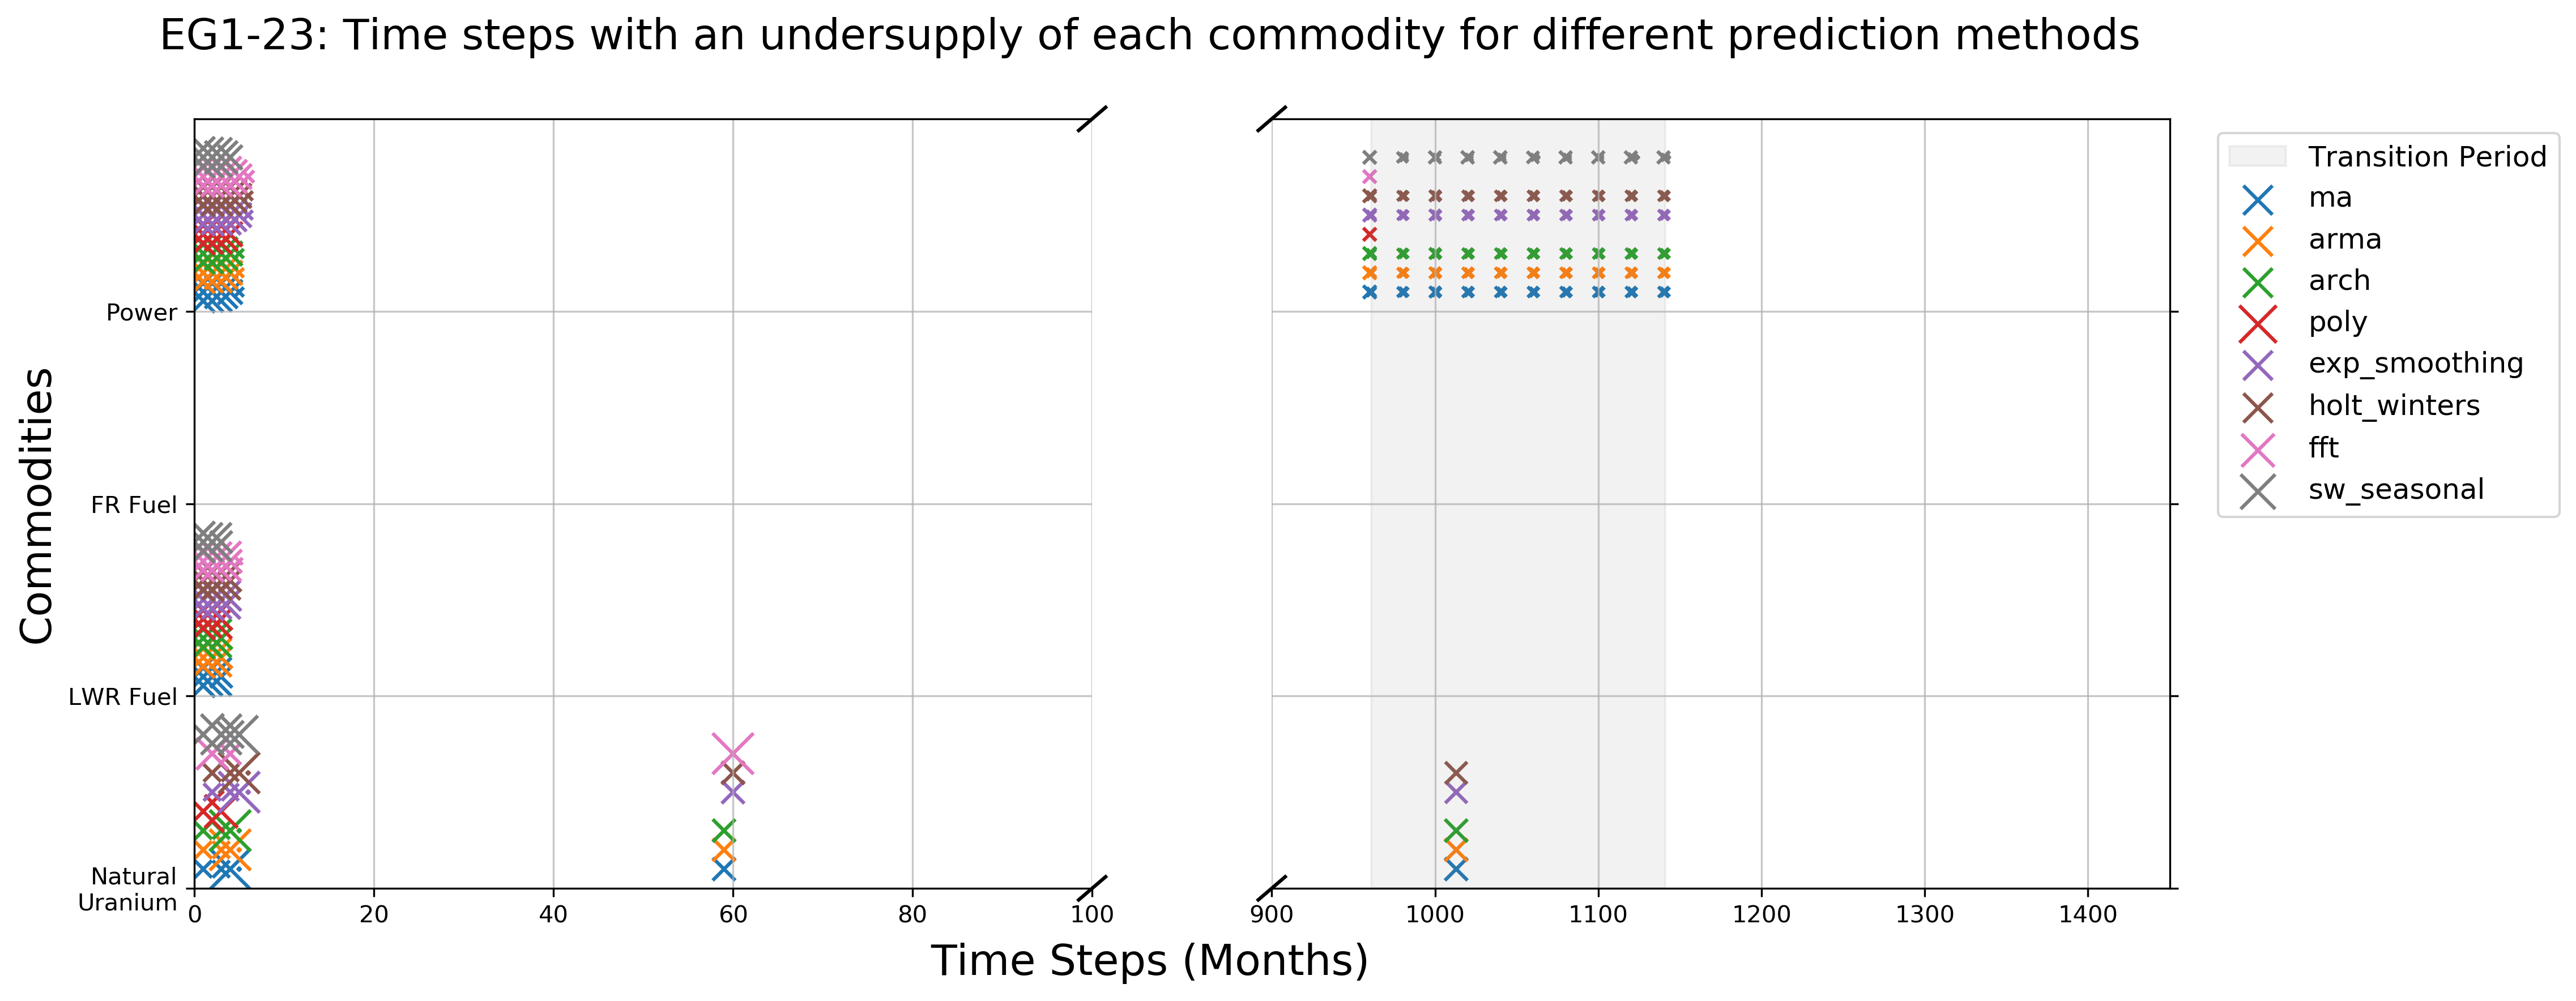
\includegraphics[width=\textwidth]{../paper/figures/eg23-undersupply.png}
    \end{center}
          \caption{Time dependent undersupply of commodities for different
          prediction methods for the EG01-23 Transition Scenario with Constant Power Demand. The
          size of each cross is based on the size of the undersupply.
          Fewer crosses on plot indicates the method is more successful at preventing undersupply 
          of each commodity}
  \end{figure}
\end{frame}

\begin{frame}
    \frametitle{Comparison of Prediction Methods}
    \textbf{EG01-23 Constant Power Demand Transition Scenario}
\begin{figure}[htbp!]
    \begin{center}
      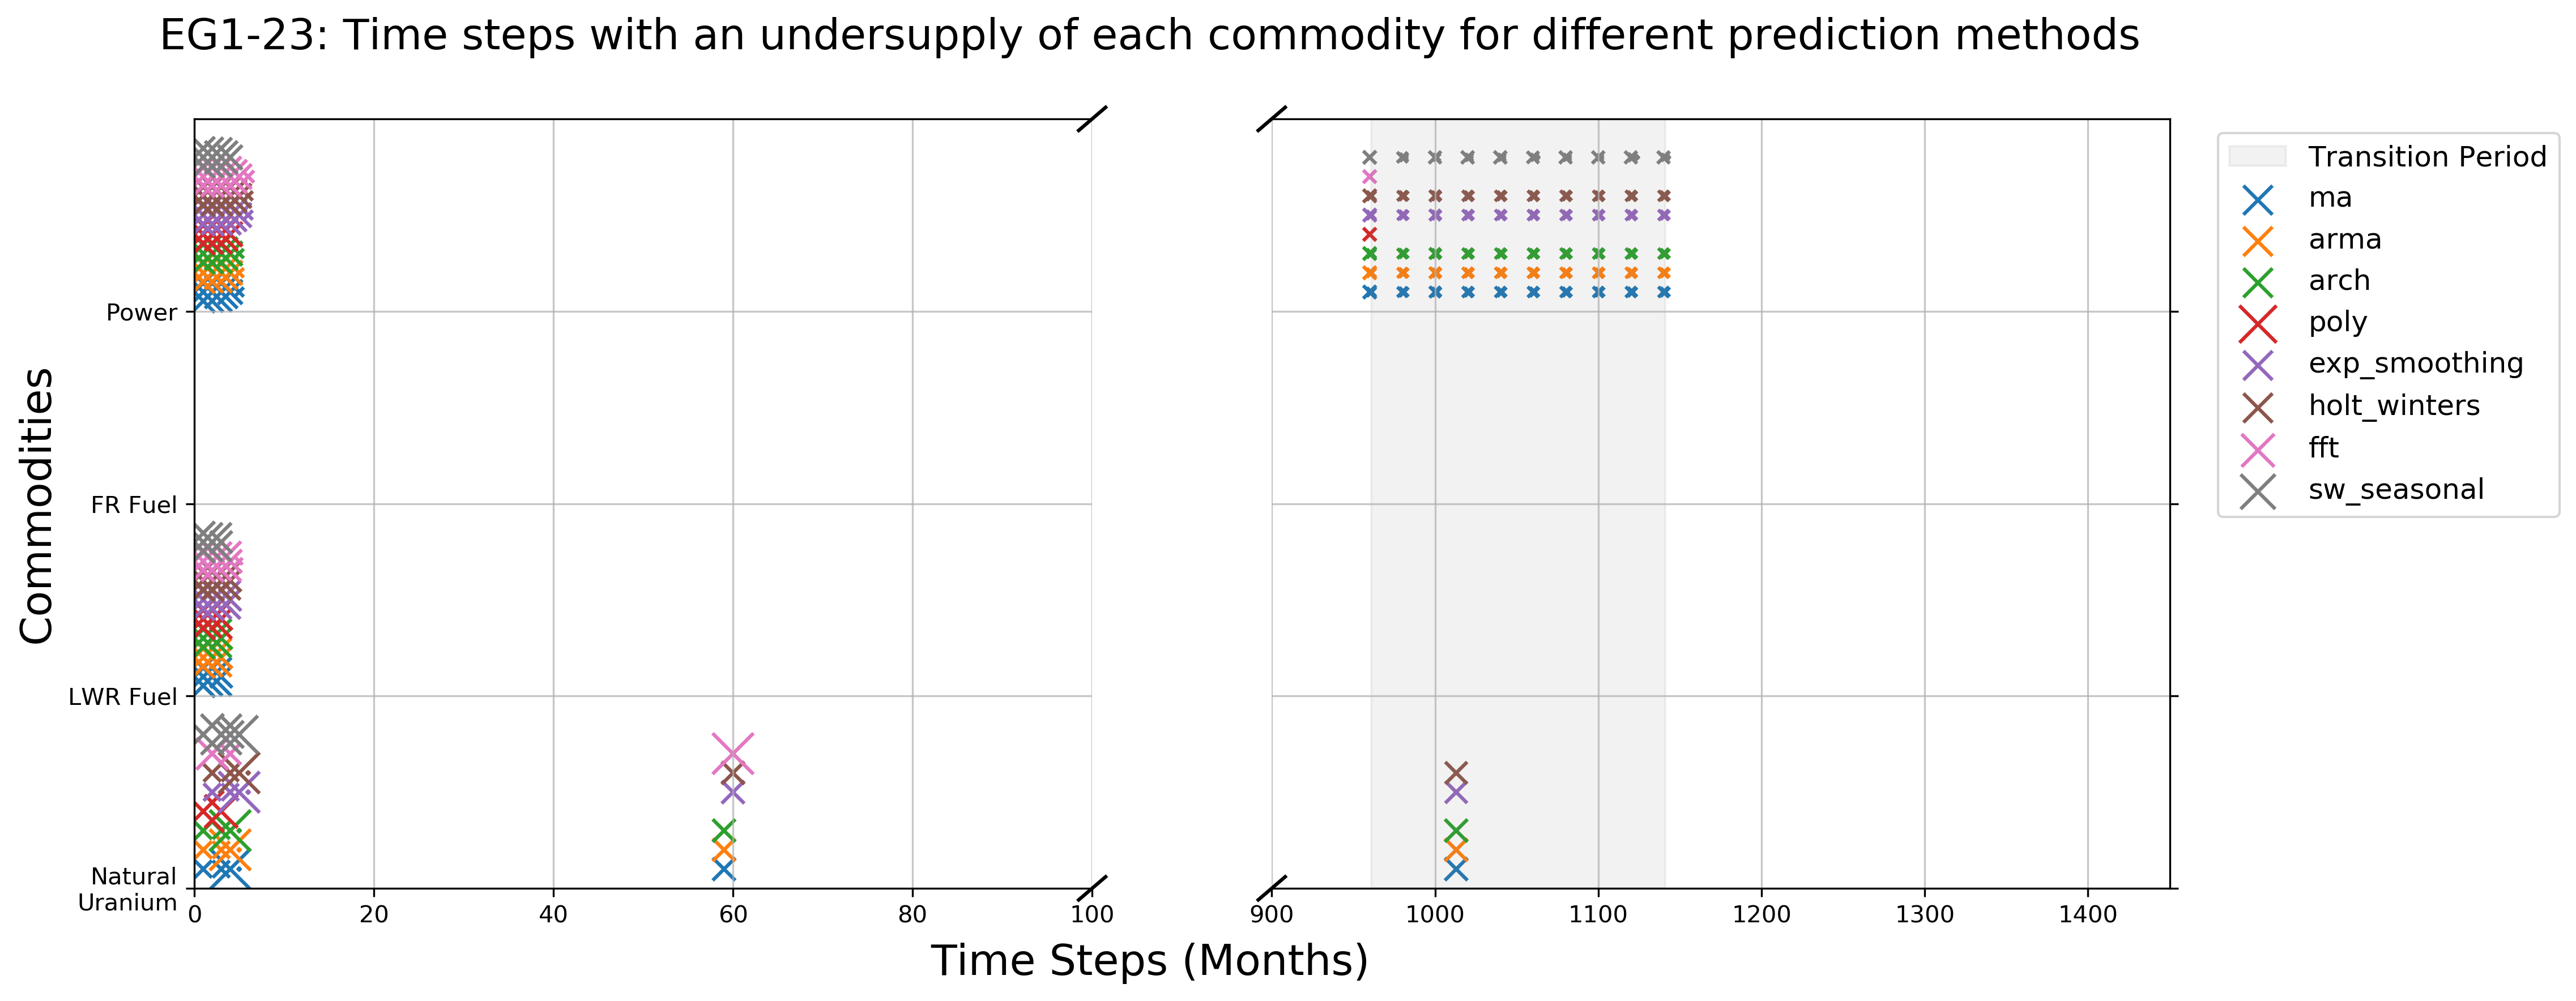
\includegraphics[width=\textwidth]{../paper/figures/eg23-undersupply.png}
    \end{center}
          \caption{Time dependent undersupply of commodities for different
          prediction methods for the EG01-23 Transition Scenario with Constant Power Demand. The
          size of each cross is based on the size of the undersupply.
          Fewer crosses on plot indicates the method is more successful at preventing under capacity 
          of each commodity}
  \end{figure}
\end{frame}

\begin{frame}
    \frametitle{Comparison of Prediction Methods}
\textbf{EG01-24 Constant Power Demand Transition Scenario}
\begin{figure}[htbp!]
    \begin{center}
      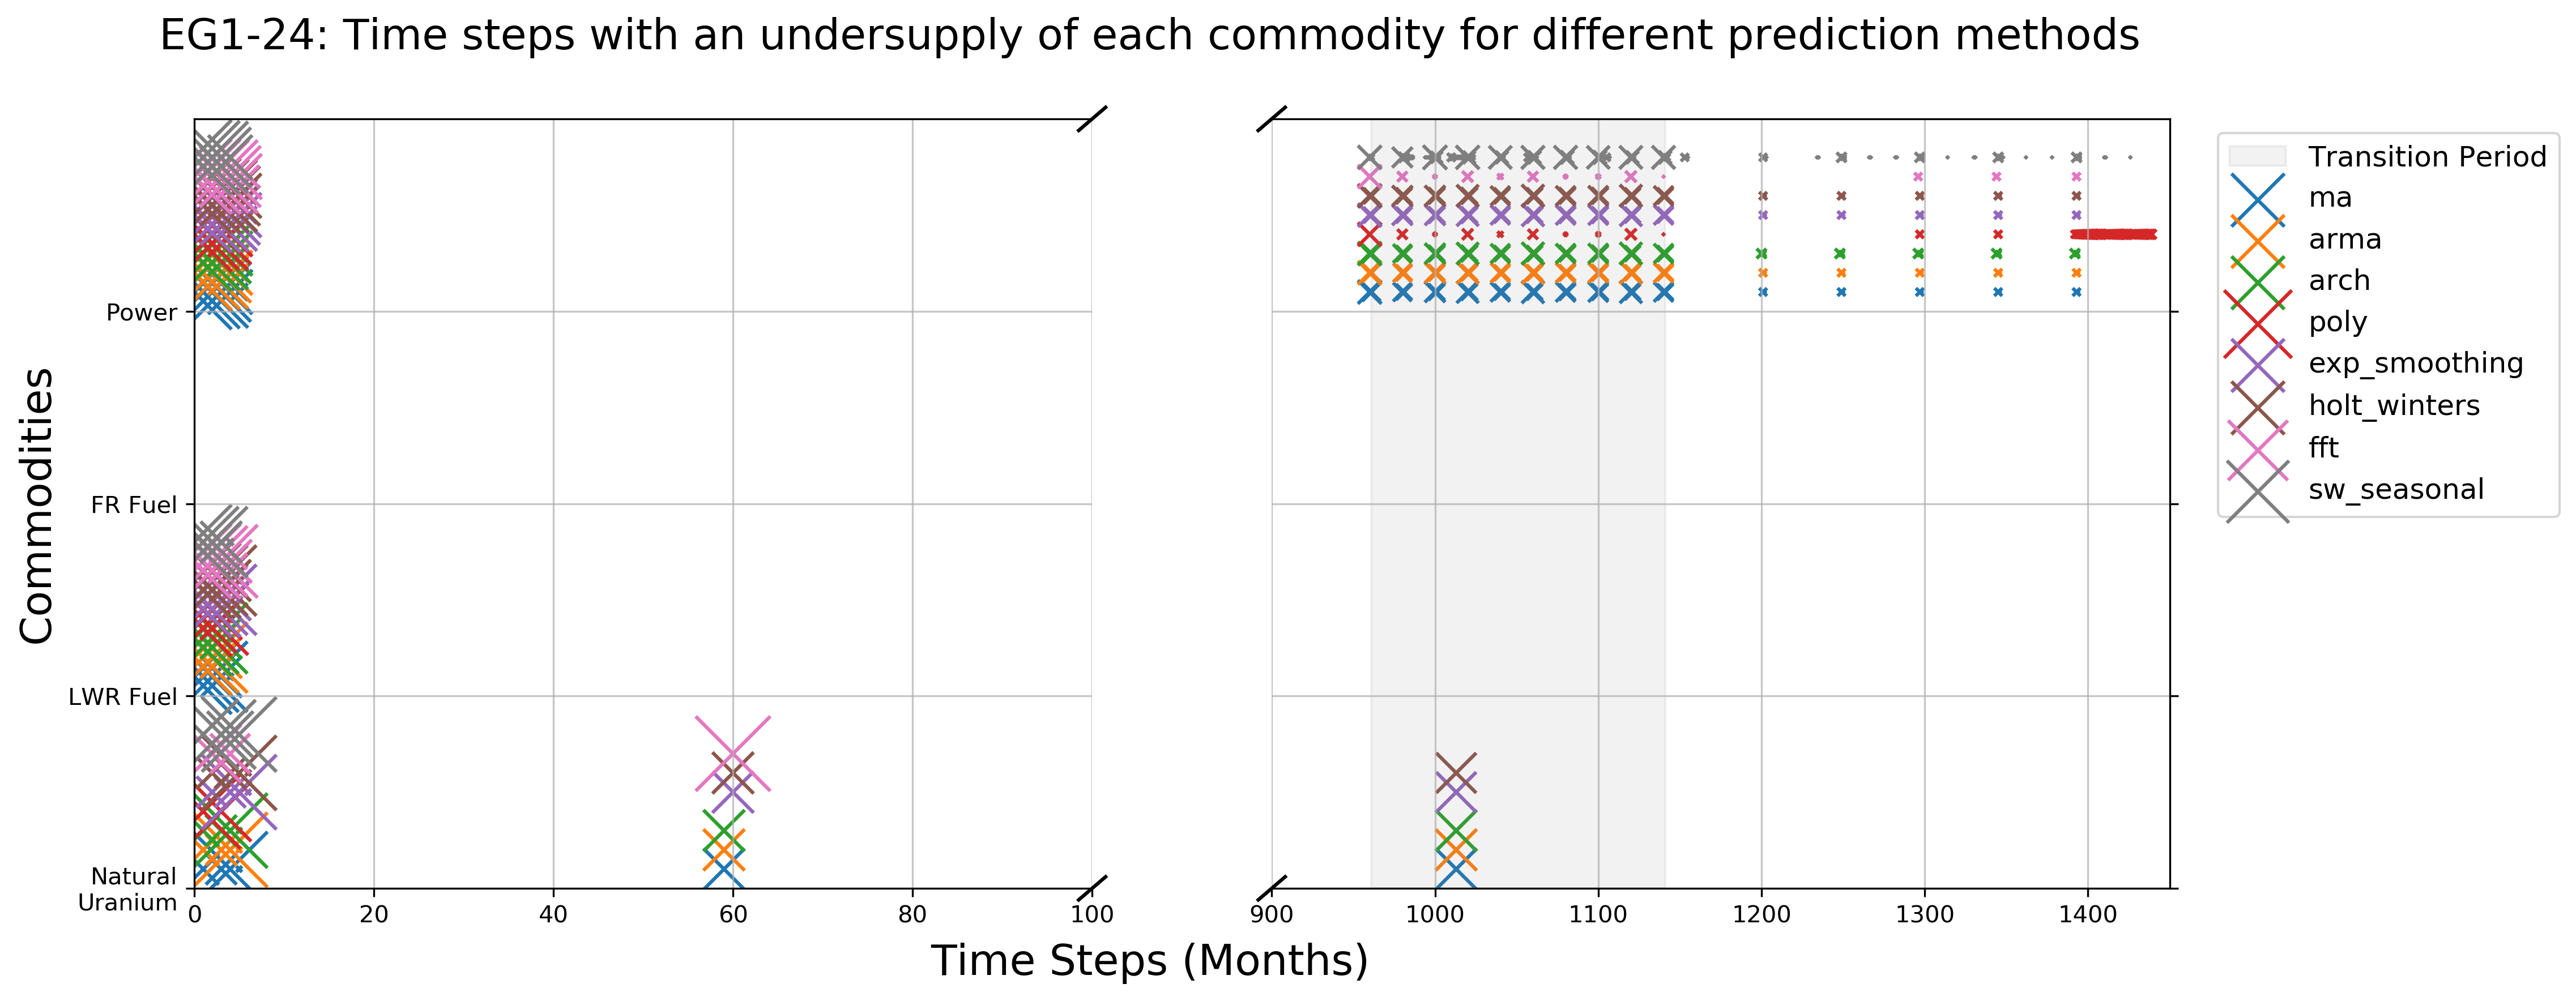
\includegraphics[width=\textwidth]{../paper/figures/eg24-undersupply.png}
    \end{center}
          \caption{Time dependent undersupply of commodities for different
          prediction methods for the EG01-24 Transition Scenario with Linearly Increasing Power Demand.The
          size of each cross is based on the size of the undersupply.
          Fewer crosses on plot indicates the method is more successful at preventing undersupply 
          of each commodity}
  \end{figure}
\end{frame}

\begin{frame}
    \frametitle{Comparison of Prediction Methods}
    \textbf{EG01-24 Constant Power Demand Transition Scenario}
\begin{figure}[htbp!]
    \begin{center}
      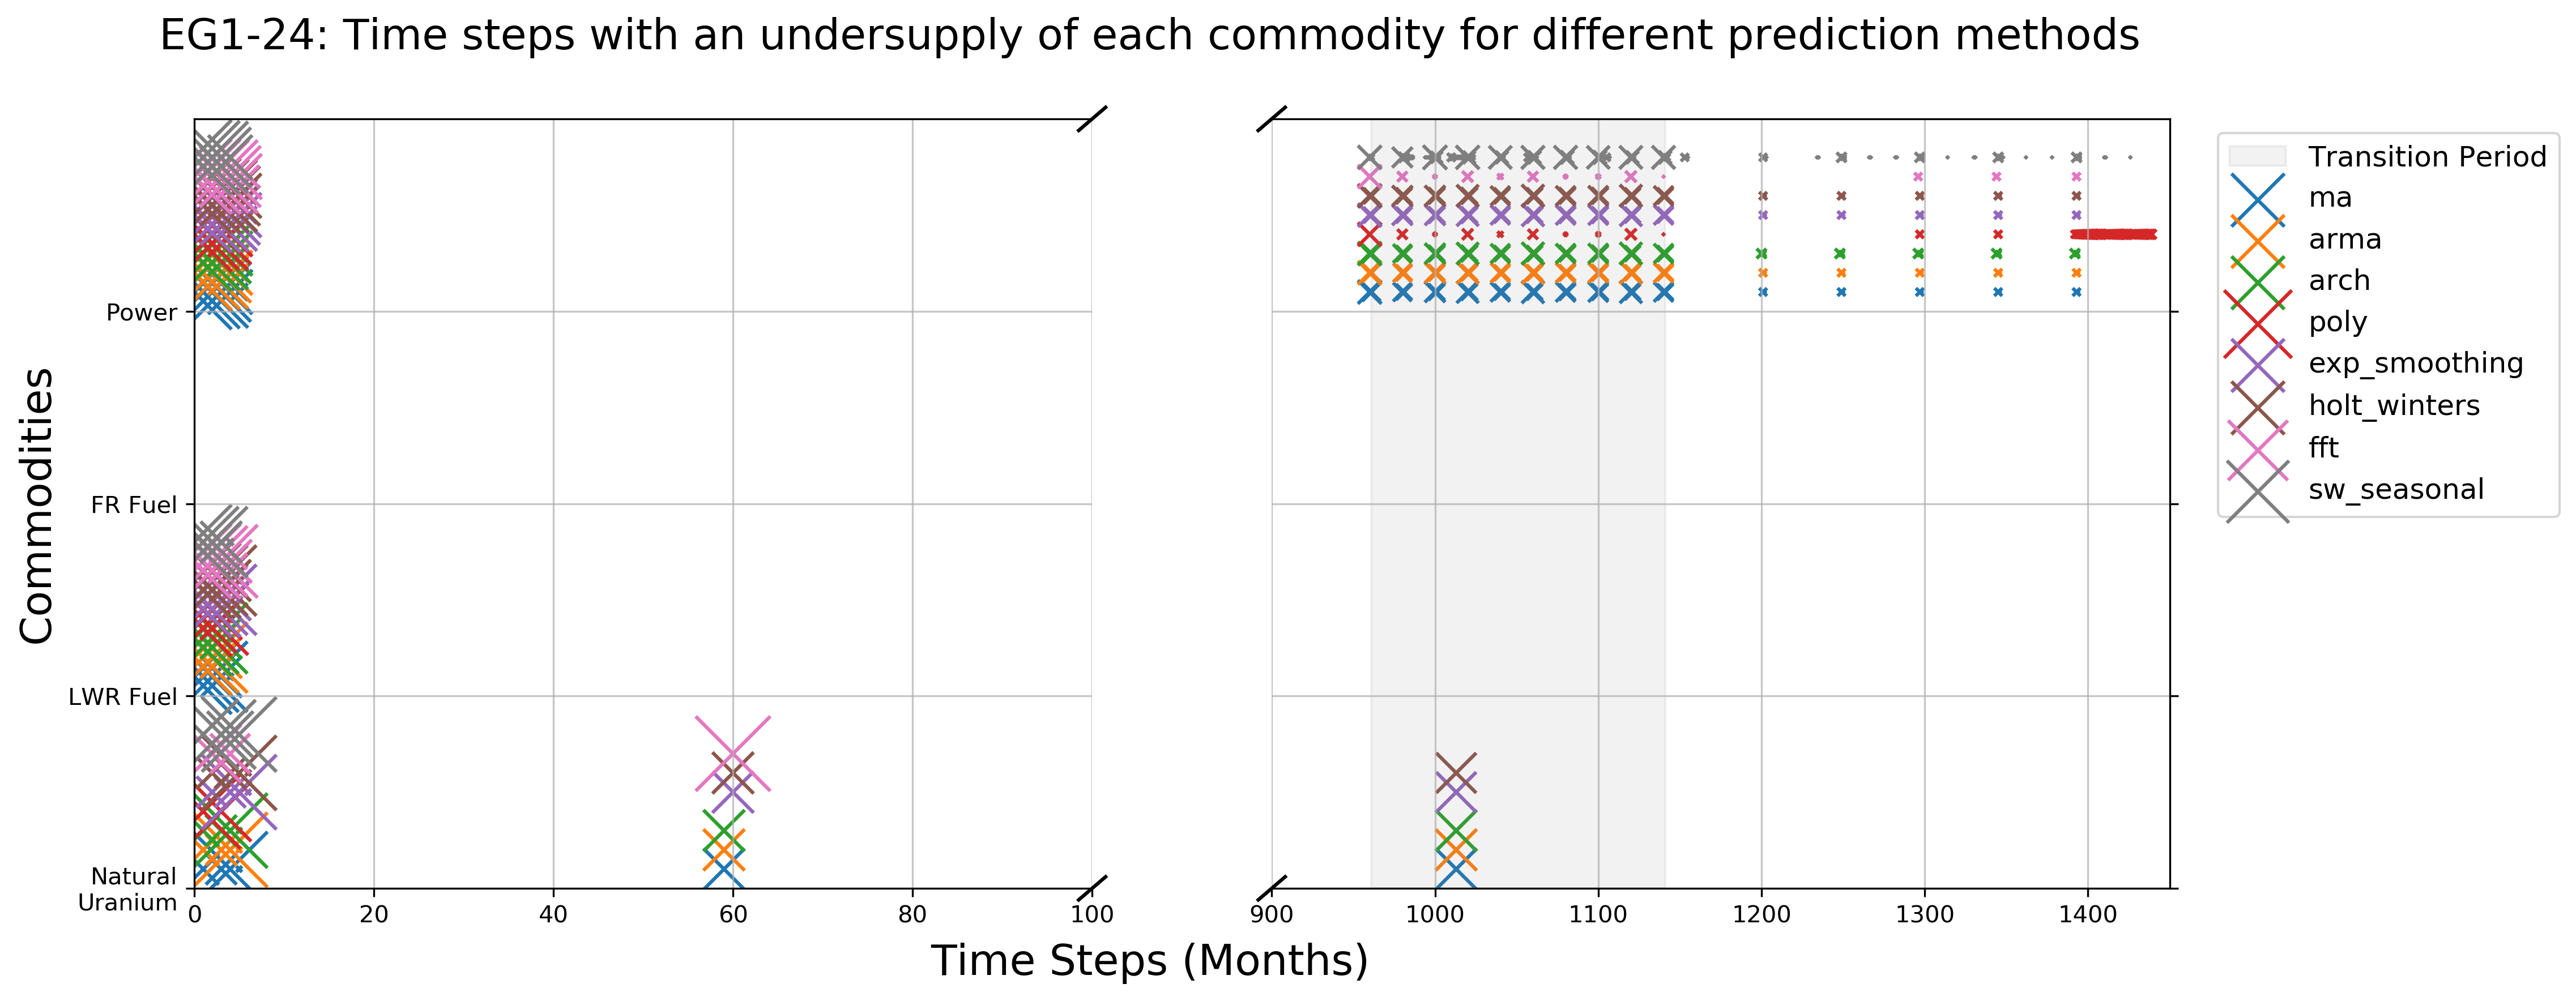
\includegraphics[width=\textwidth]{../paper/figures/eg24-undersupply.png}
    \end{center}
          \caption{Time dependent undersupply of commodities for different
          prediction methods for the EG01-24 Transition Scenario with Linearly Increasing Power Demand. The
          size of each cross is based on the size of the under capacity.
          Fewer crosses on plot indicates the method is more successful at preventing under capacity
          of each commodity}
  \end{figure}
\end{frame}

\begin{frame}
  \frametitle{Comparison of Prediction Methods}
  \textbf{Main Takeaway}
  \\
  The best performing prediction method for each transition scenario is: 
  \begin{enumerate}
    \item EG01-23 Constant Power Demand: Polynomial Fit 
    \item EG01-24 Linearly Increasing Power Demand: Fast Fourier Transform
    \item EG01-29 Constant Power Demand: Polynomial Fit 
    \item EG01-30 Linearly Increasing Power Demand: Fast Fourier Transform
\end{enumerate}
\end{frame}
\subsection{Sensitivity Analysis of Power Buffer Size}
\begin{frame}
    \frametitle{Sensitivity Analysis of Power Buffer}
    \textbf{EG01-24}: Linearly Increasing Power Demand
    \begin{figure}[htbp!]
        \begin{center}
          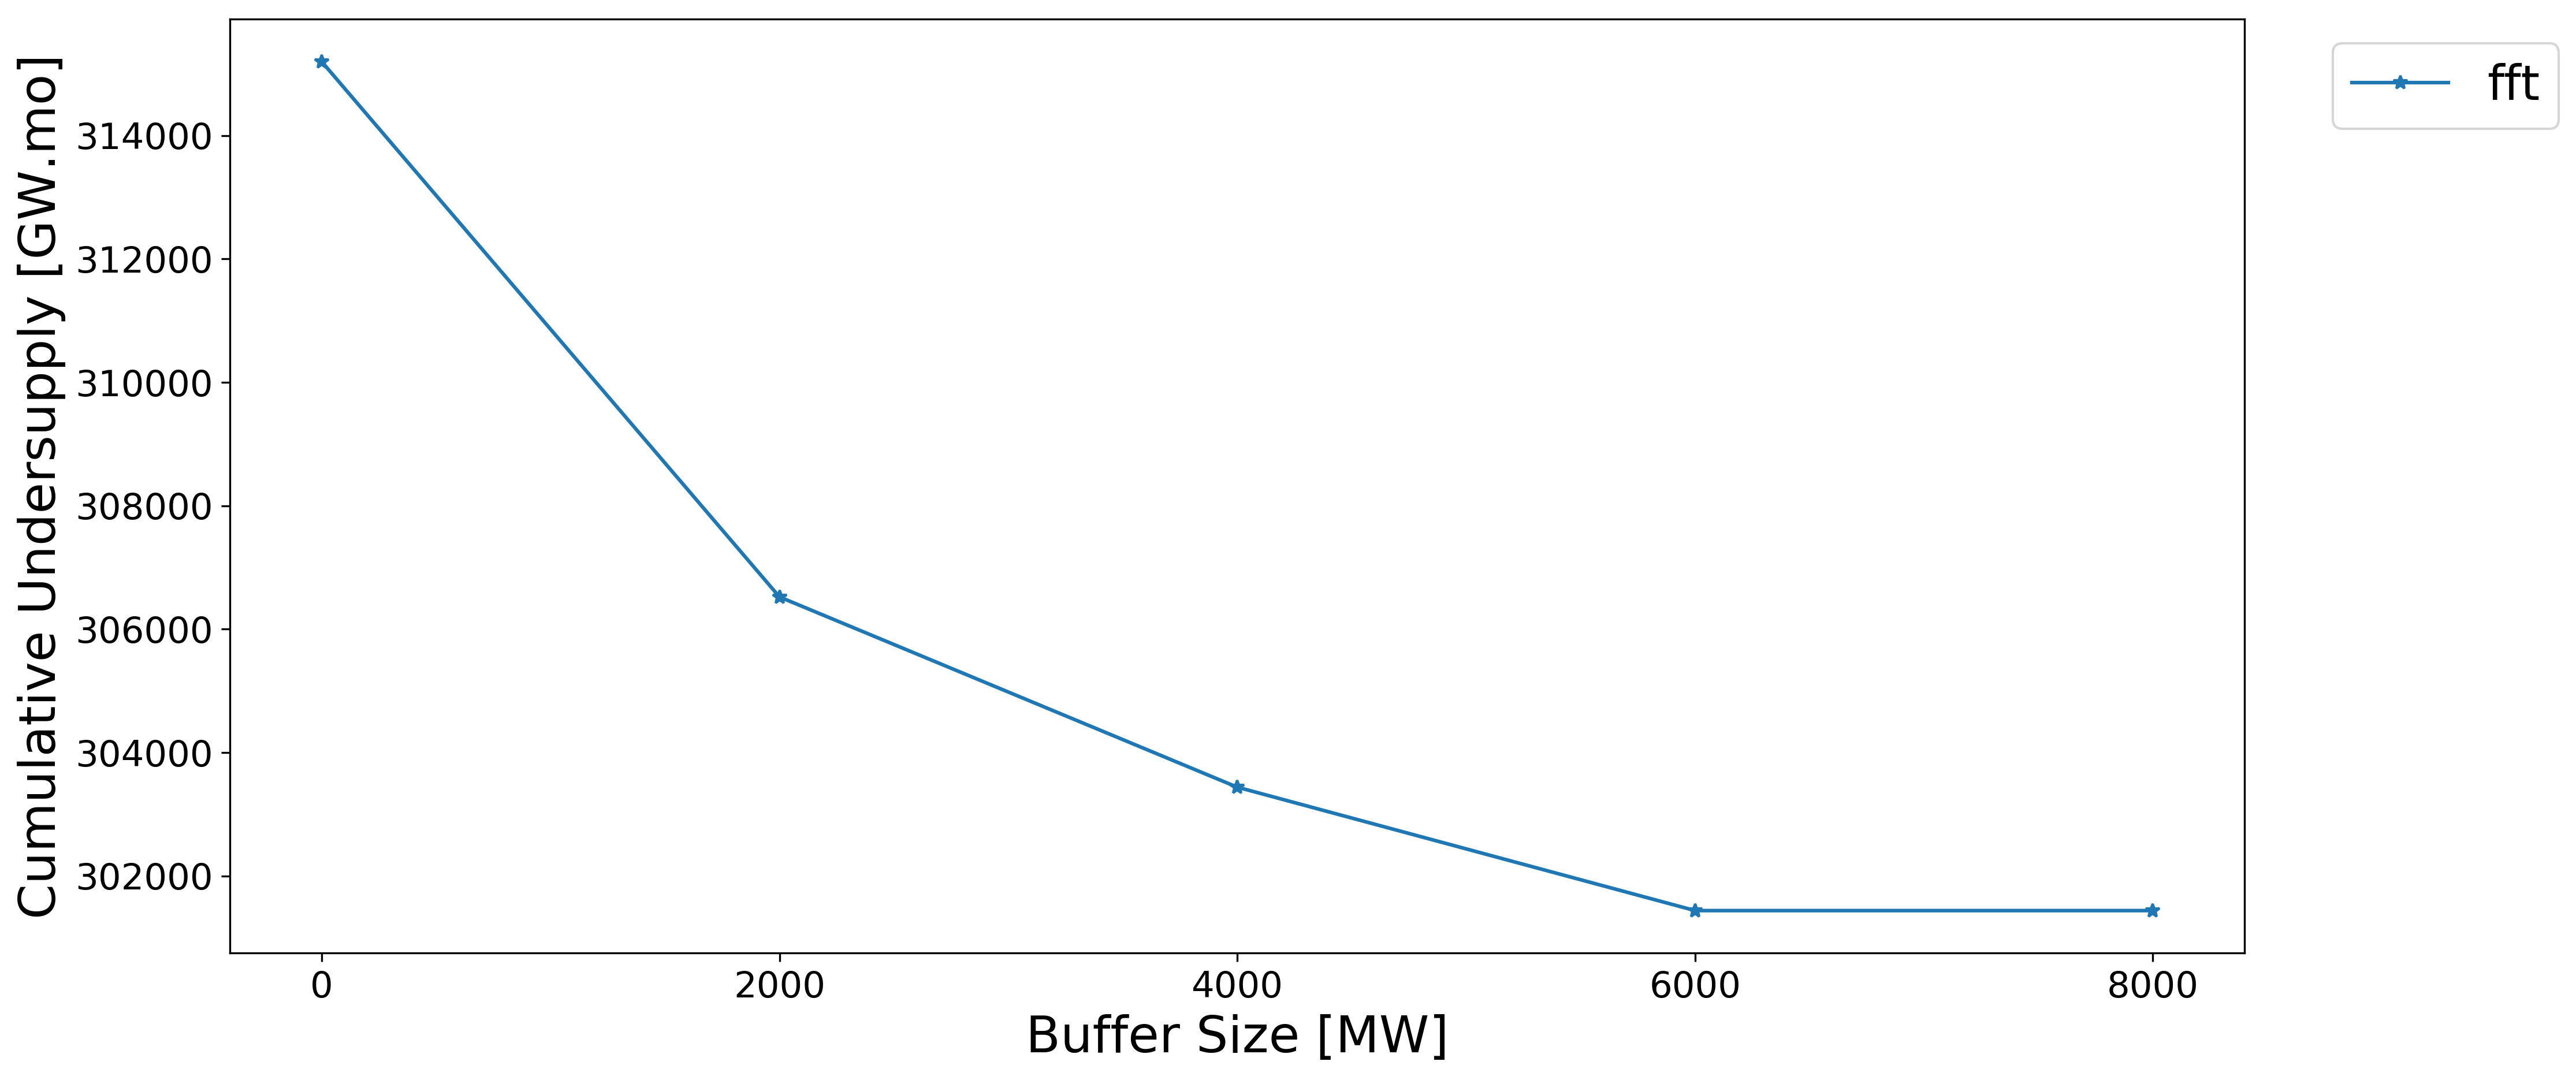
\includegraphics[width=0.8\textwidth]{../paper/figures/24-sens-buffer}
        \end{center}
              \caption{Sensitivity Analysis of Power buffer size on cumulative 
              undersupply of Power for EG01-EG24 transition scenarios 
              with linearly increasing power demand using the fft prediction method.}
      \end{figure}
\end{frame}

\begin{frame}
    \frametitle{Sensitivity Analysis of Power Buffer}
    \textbf{EG01-30}: Linearly Increasing Power Demand
    \begin{figure}[htbp!]
        \begin{center}
          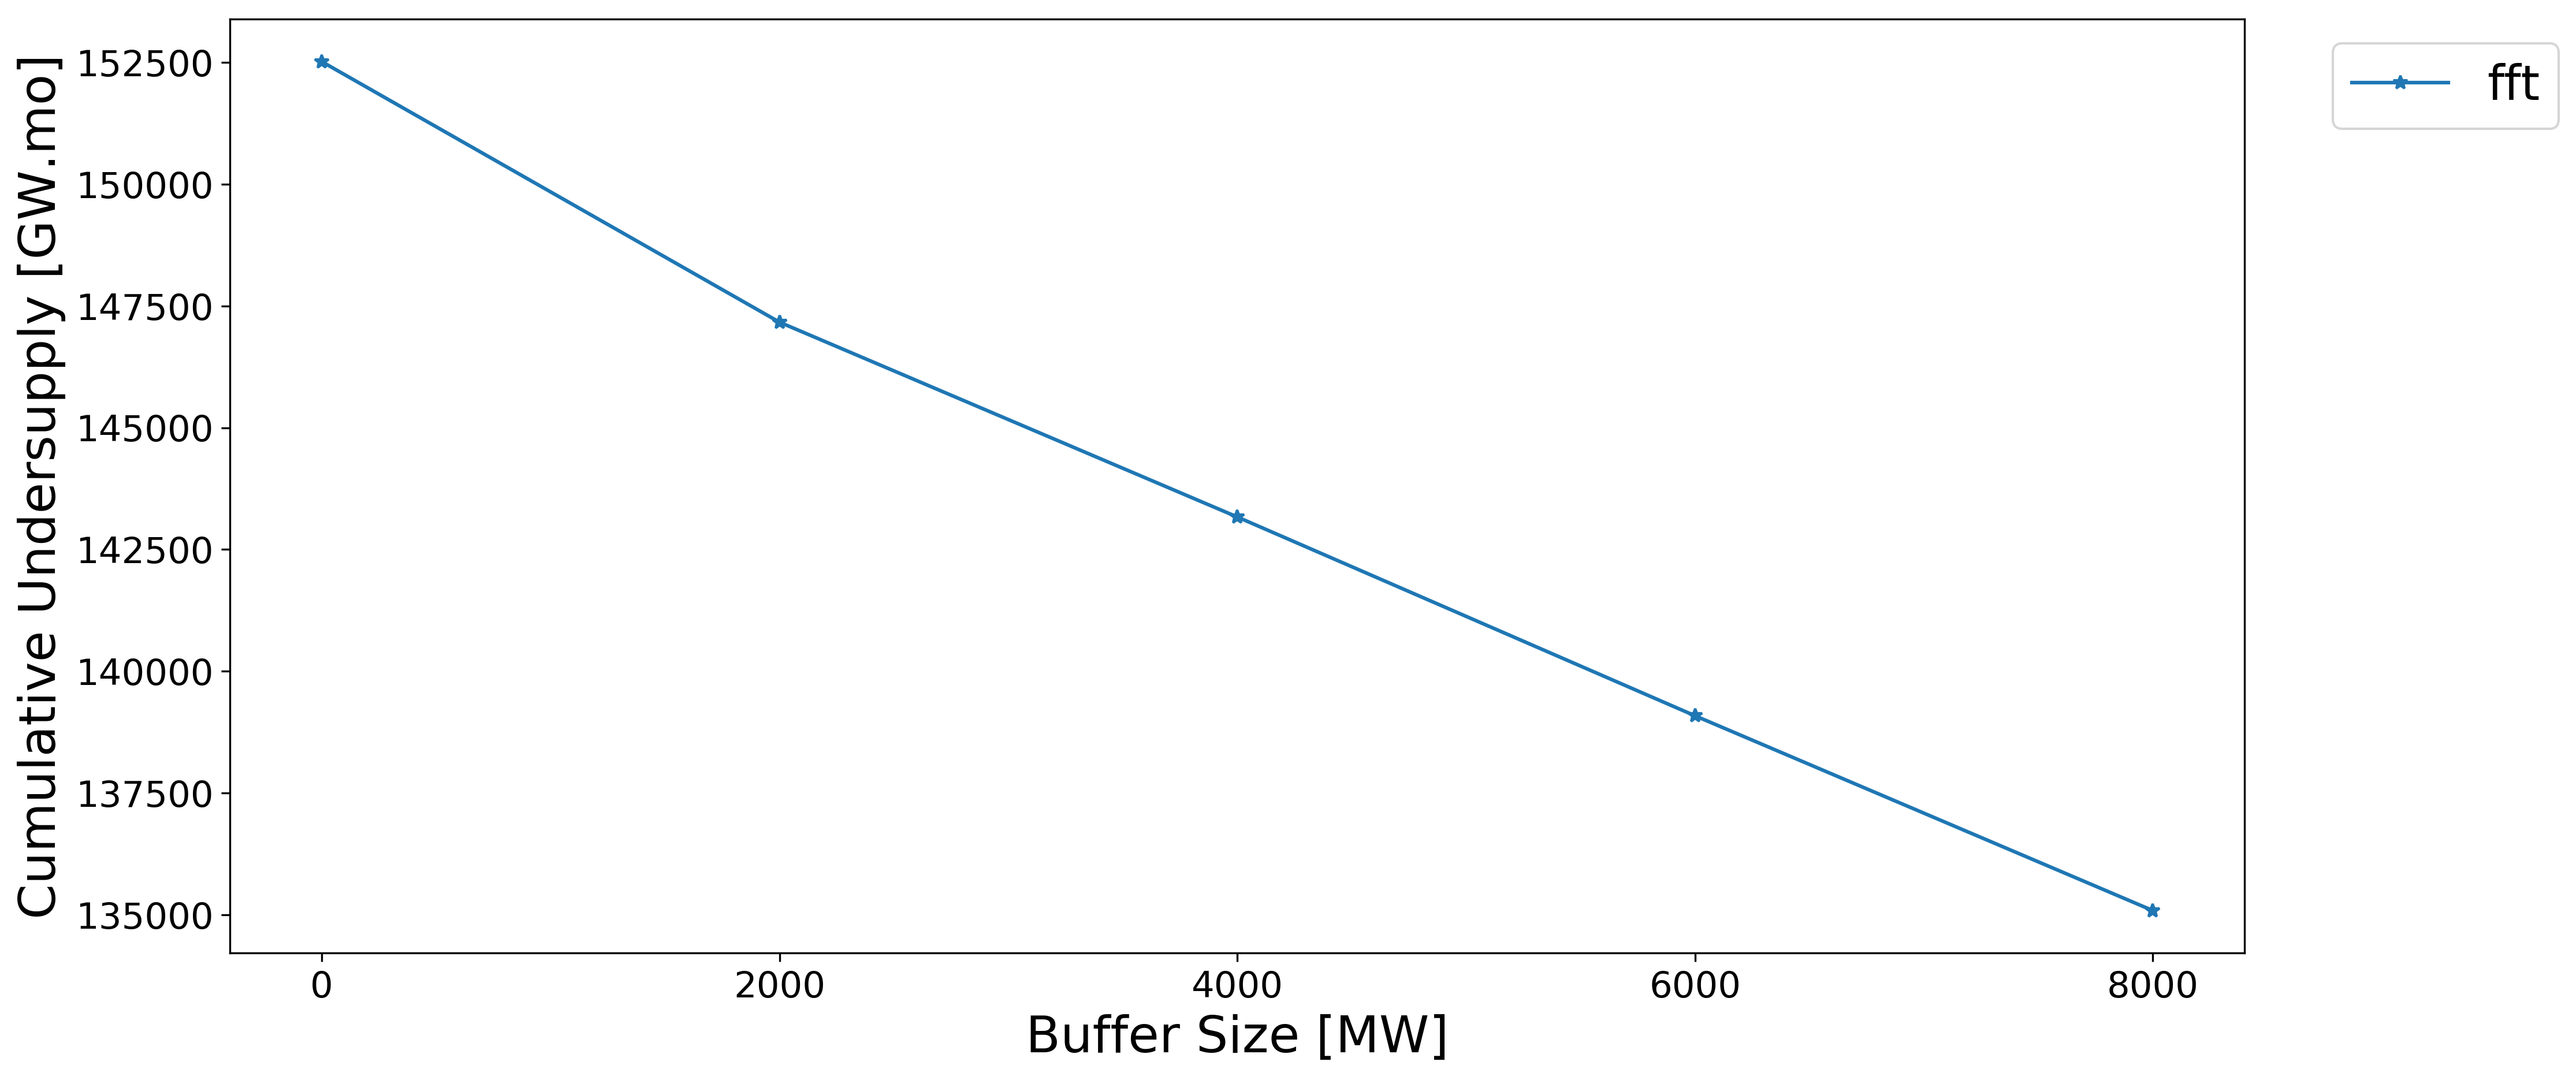
\includegraphics[width=0.8\textwidth]{../paper/figures/30-sens-buffer}
        \end{center}
              \caption{Sensitivity Analysis of Power buffer size on cumulative 
              undersupply of Power for EG01-EG30 transition scenarios 
              with linearly increasing power demand using the fft prediction method.}
      \end{figure}
\end{frame}

\begin{frame}
  \frametitle{Sensitivity Analysis of Power Buffer}
  \textbf{Main Takeaway}
  \\
  The best power supply buffer for each transition scenario is: 
  \begin{enumerate}
    \item EG01-23 Constant Power Demand: 0 MW
    \item EG01-24 Linearly Increasing Power Demand: 6000 MW
    \item EG01-29 Constant Power Demand: 0 MW
    \item EG01-30 Linearly Increasing Power Demand: 8000 MW 
\end{enumerate}
\end{frame}
\subsection{Best Performing Transition Scenarios}
\begin{frame}
    \frametitle{Best Performing Transition Scenarios}
    \textbf{Input Parameters of best performing transition scenarios}
    \begin{table}[]
      {\renewcommand{\arraystretch}{1.2}
        \resizebox{\textwidth}{!}{%
        \begin{tabular}{l|l|c|l|l|l}
        \hline
        \multirow{2}{*}{}                         & \multicolumn{1}{c|}{\multirow{2}{*}{\textbf{Input Parameter}}} & \multicolumn{4}{c}{\textbf{Simulation Description}}                                                                                                                                                                                                                                                       \\ \cline{3-6} 
                                                  & \multicolumn{1}{c|}{}                                          & \multicolumn{1}{l|}{\textbf{EG01-23}}                                                                 & \textbf{EG01-24}                  & \textbf{EG01-29}                 &\textbf{EG01-30}                                                  \\ \hline
        \multirow{4}{*}{\textbf{Required}} & Demand driving commodity                                       & \multicolumn{4}{c}{Power}                                                                                                                                                                                                                                                                                 \\ \cline{2-6} 
                                                  & Demand equation [MW]                                               & \multicolumn{1}{l|}{60000}                                                                                & $60000 + 250t/12$ & 60000                     &     $60000 + 250t/12$                                       \\ \cline{2-6} 
                                                  & Prediction method                                              & \texttt{poly}       & \texttt{fft}             & \texttt{poly}         &  \texttt{fft}    \\ \cline{2-6} 
                                                  & Deployment Driving Method                                      & \multicolumn{4}{c}{Installed Capacity}                                                                                                                                                                                                                                                                    \\ \hline
        \multirow{2}{*}{\textbf{Optional}} & Buffer type                                                    & \multicolumn{4}{c}{Absolute}                                                                                                                                                                                                                                                               \\ \cline{2-6} 
                                                  & Power Buffer size [MW]                                                   & 0 & 6000 & 0 & 8000 \\ \hline
        \end{tabular}%
        }}
        \caption{\deploy's input parameters for all 4 transition scenarios
        that minimizes undersupply of power and minimizes 
        the undersupply and under capacity of the other facilities. }
        \label{tab:bestinputs}
        \end{table}
\end{frame}

\begin{frame}
    \frametitle{Best Performing Transition Scenarios}
    \textbf{EG01-23: Constant Power Demand}
    \begin{figure}[htbp!]
        \begin{center}
          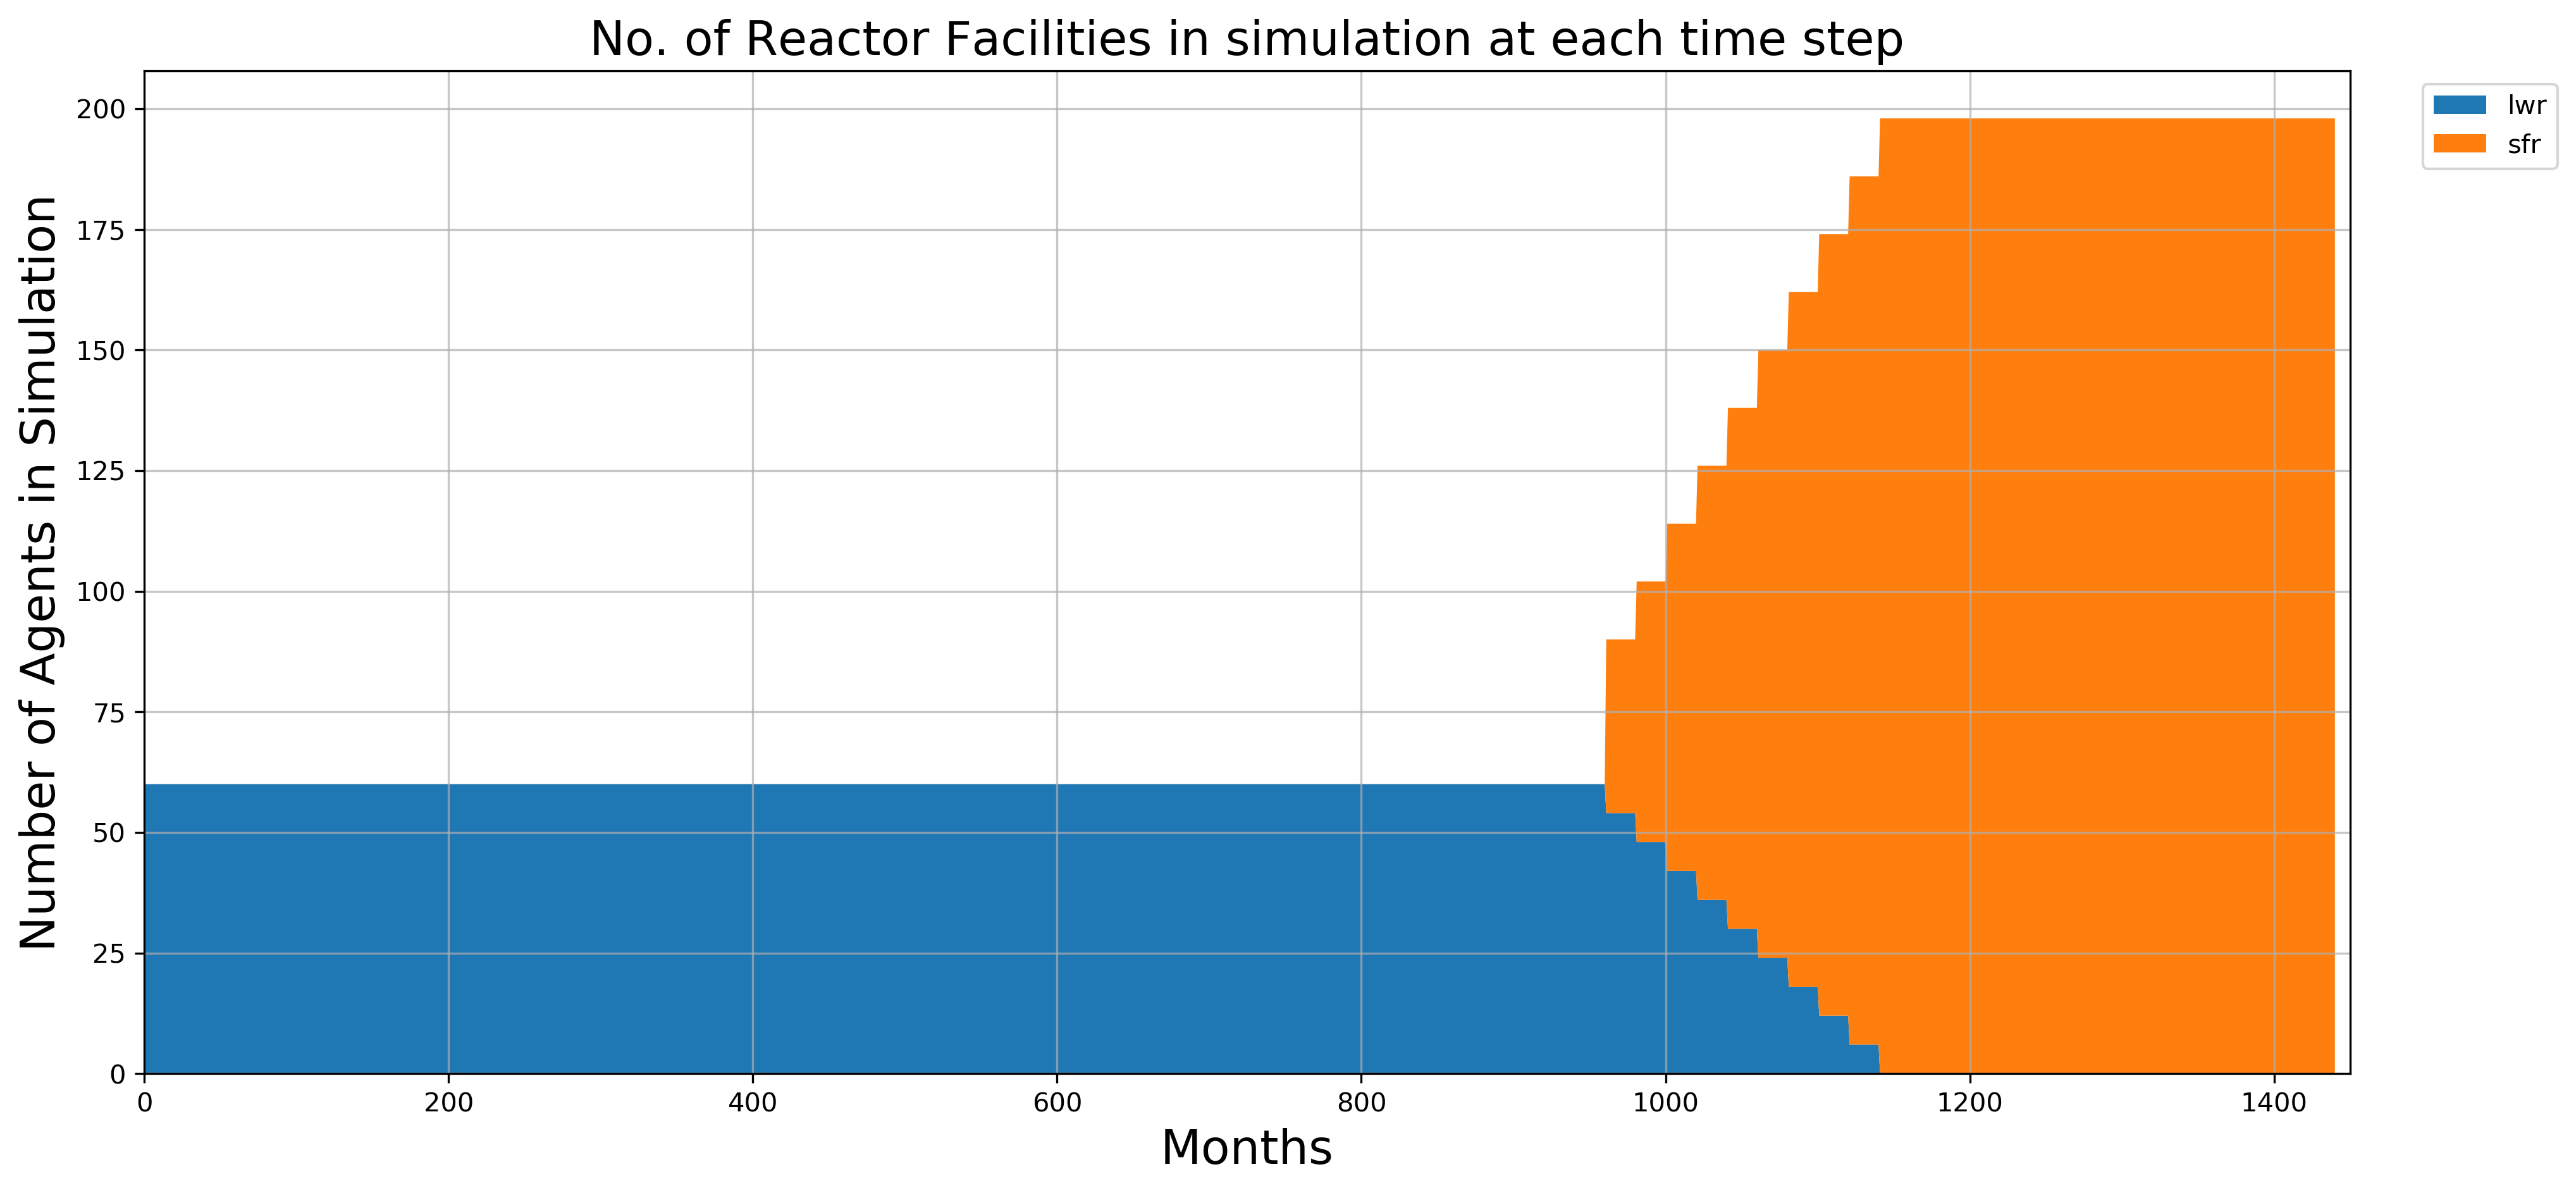
\includegraphics[width=\textwidth]{../paper/figures/eg23-stack_reactor.png}
        \end{center}
              \caption{Time dependent deployment of reactor facilities in 
              the EG01-23 constant power demand transition scenario. 
              \deploy automatically deploys reactor facilities 
              to set up a supply chain to meet constant power demand of $60000$ MW
              during a transition from \glspl{LWR} to \glspl{SFR}. Note: \glspl{SFR}
              in this simulation have $\frac{1}{3}$ power capacity of \glspl{PWR}.}.
      \end{figure}
\end{frame}

\begin{frame}
    \frametitle{Best Performing Transition Scenarios}
    \textbf{EG01-23: Constant Power Demand}
    \begin{figure}[htbp!]
        \begin{center}
          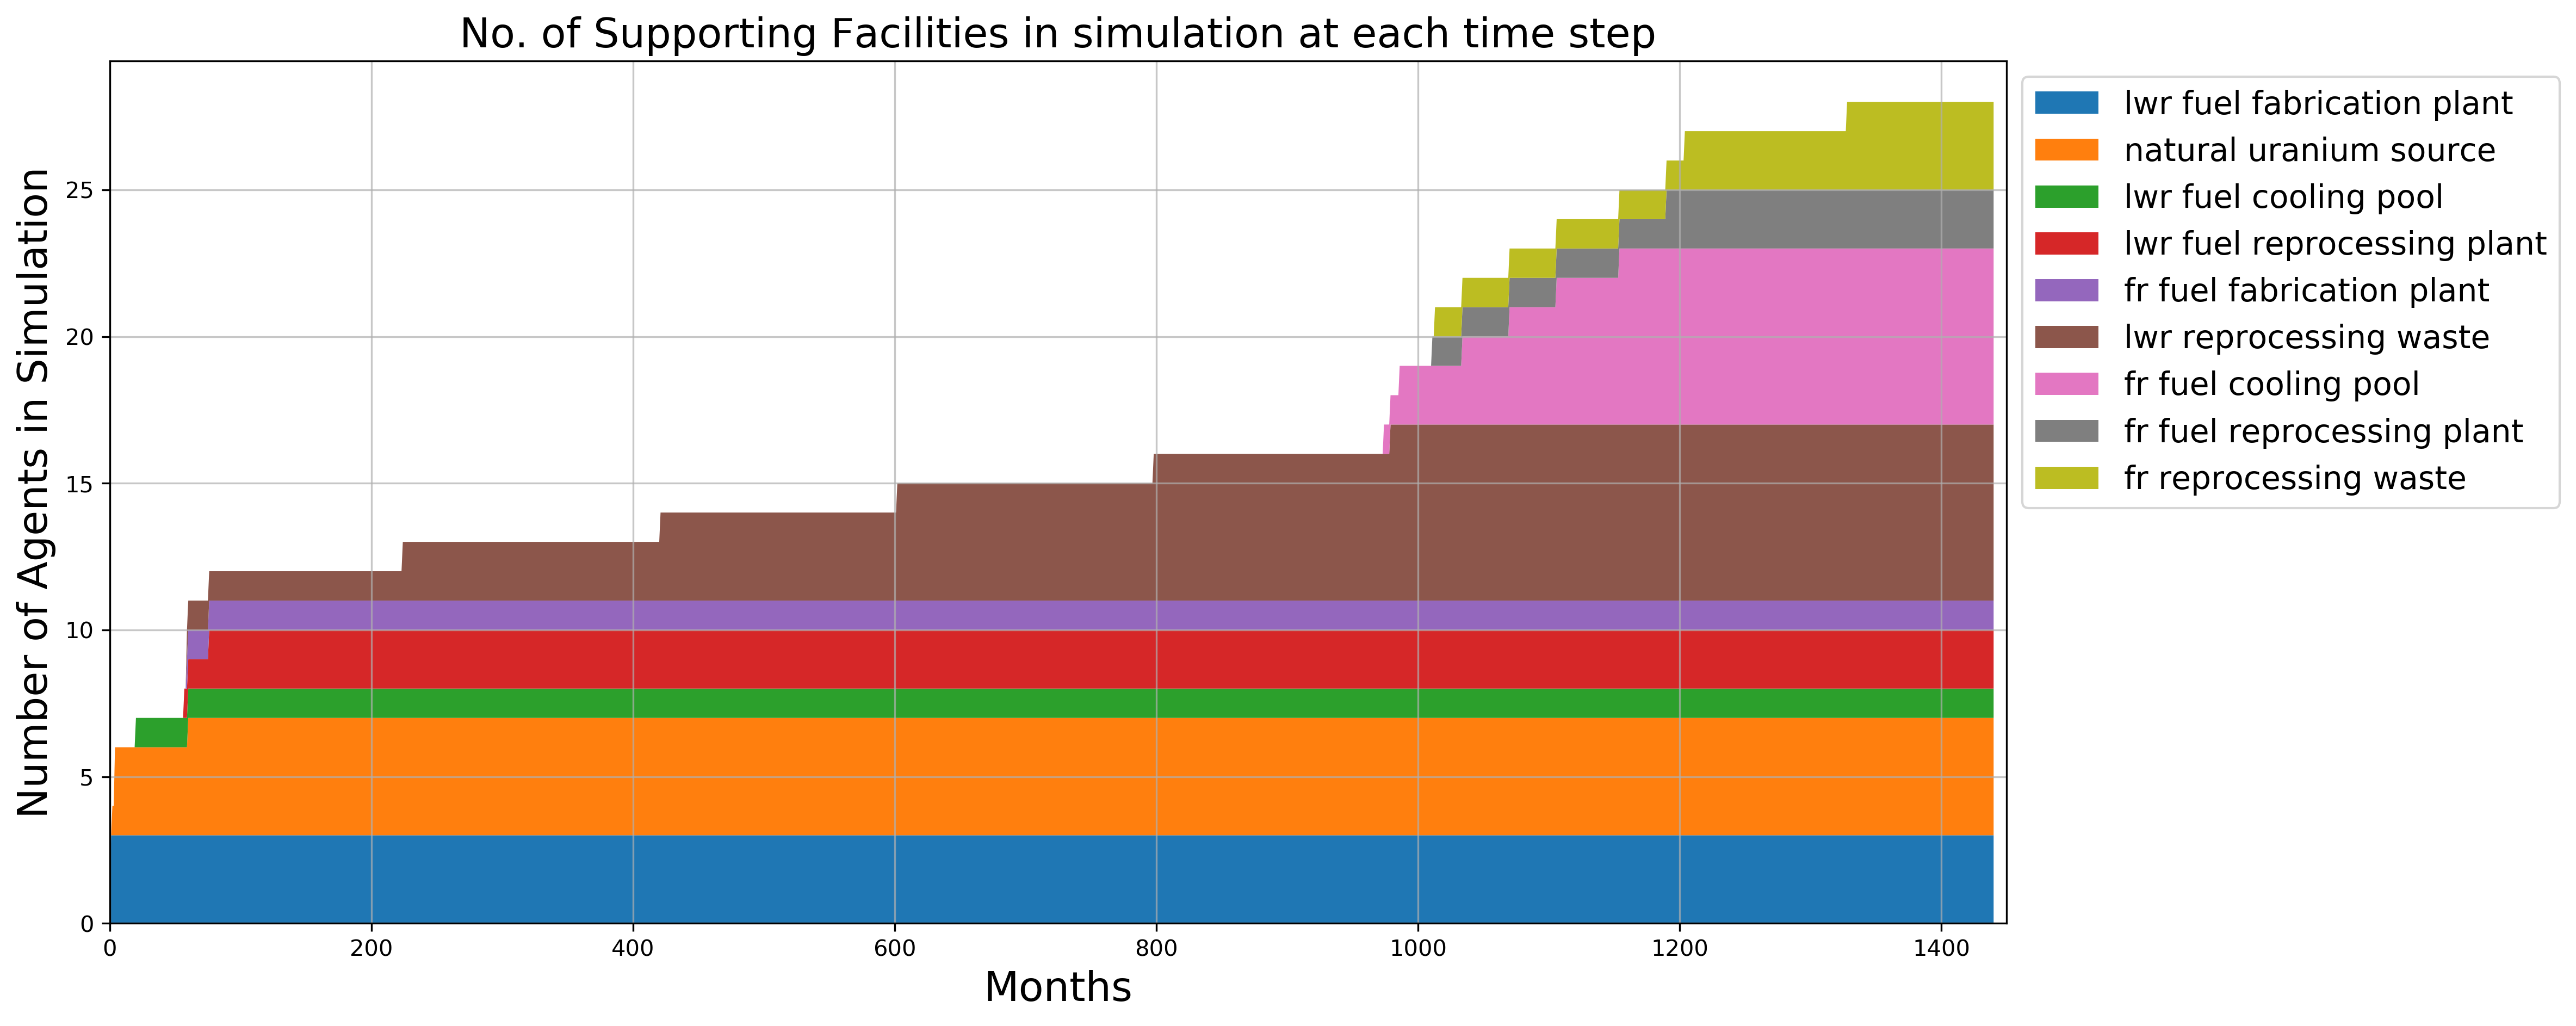
\includegraphics[width=\textwidth]{../paper/figures/eg23-stack_support.png}
        \end{center}
              \caption{Time dependent deployment of supporting facilities in 
              the EG01-23 constant power demand transition scenario. 
              \deploy automatically deploys reactor facilities 
              to set up a supply chain to meet constant power demand of $60000$ MW
              during a transition from \glspl{LWR} to \glspl{SFR}.}
      \end{figure}
\end{frame}

\begin{frame}
    \frametitle{Best Performing Transition Scenarios}
    \textbf{EG01-30: Linearly Increasing Power Demand}
    \begin{figure}[htbp!]
        \begin{center}
          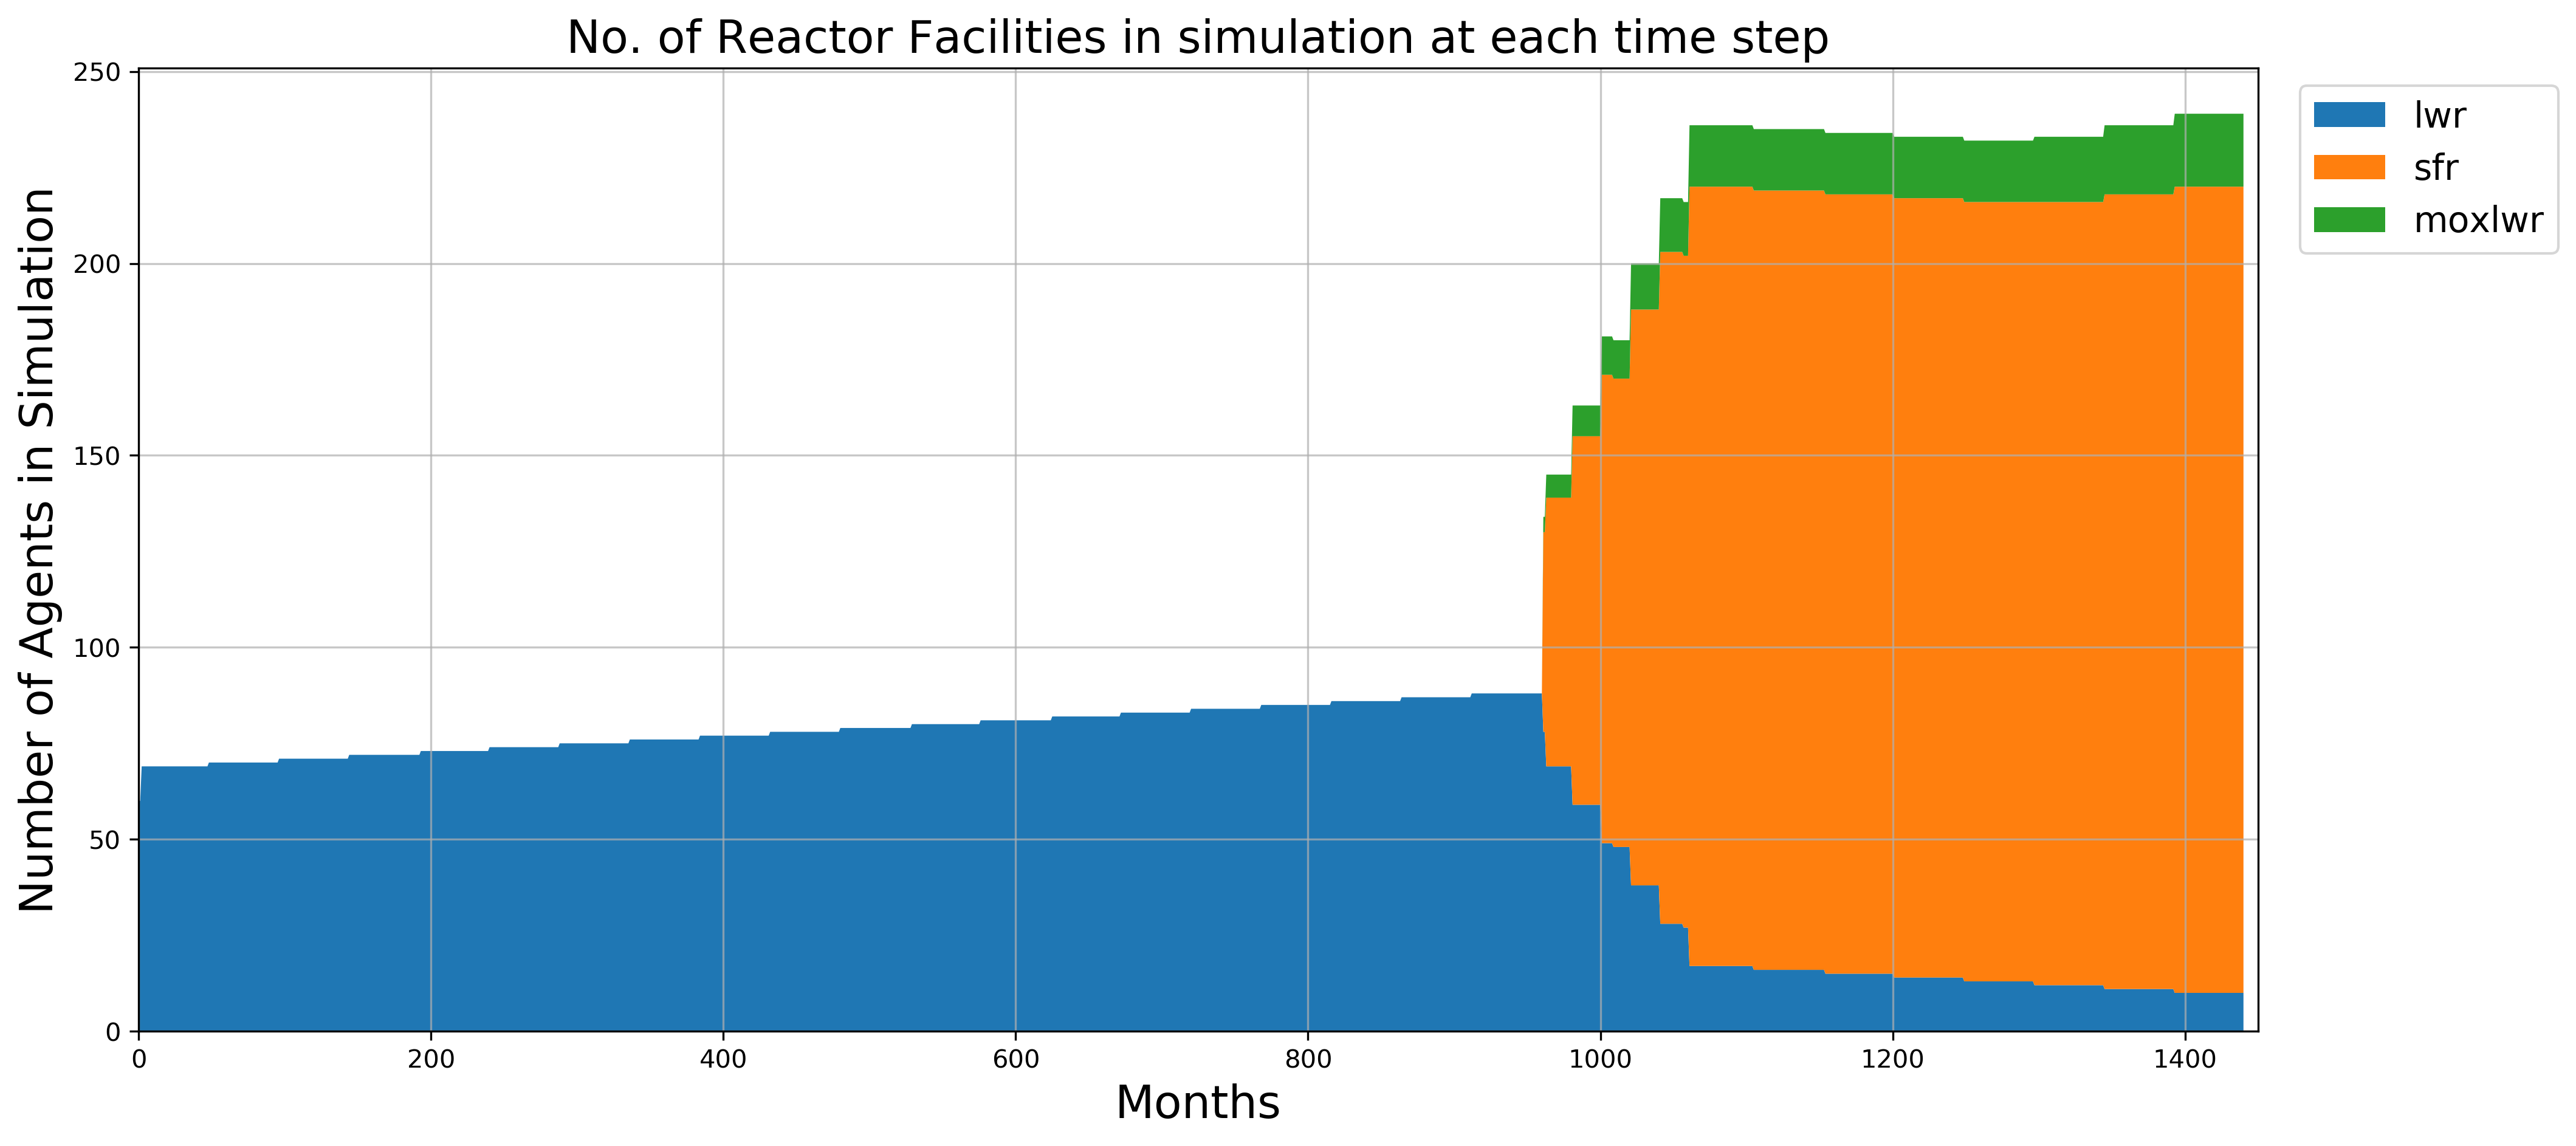
\includegraphics[width=\textwidth]{../paper/figures/eg30-stack_reactor.png}
        \end{center}
              \caption{Time dependent deployment of reactor facilities in 
              the EG01-30 linearly increasing power demand transition scenario. 
              \deploy automatically deploys reactor facilities 
              to set up a supply chain to meet constant power demand of $60000+250t/12$ MW
              during a transition from \glspl{LWR} to \glspl{SFR}.}
      \end{figure}
\end{frame}

\begin{frame}
    \frametitle{Best Performing Transition Scenarios}
    \textbf{EG01-30: Linearly Increasing Power Demand}
    \begin{figure}[htbp!]
        \begin{center}
          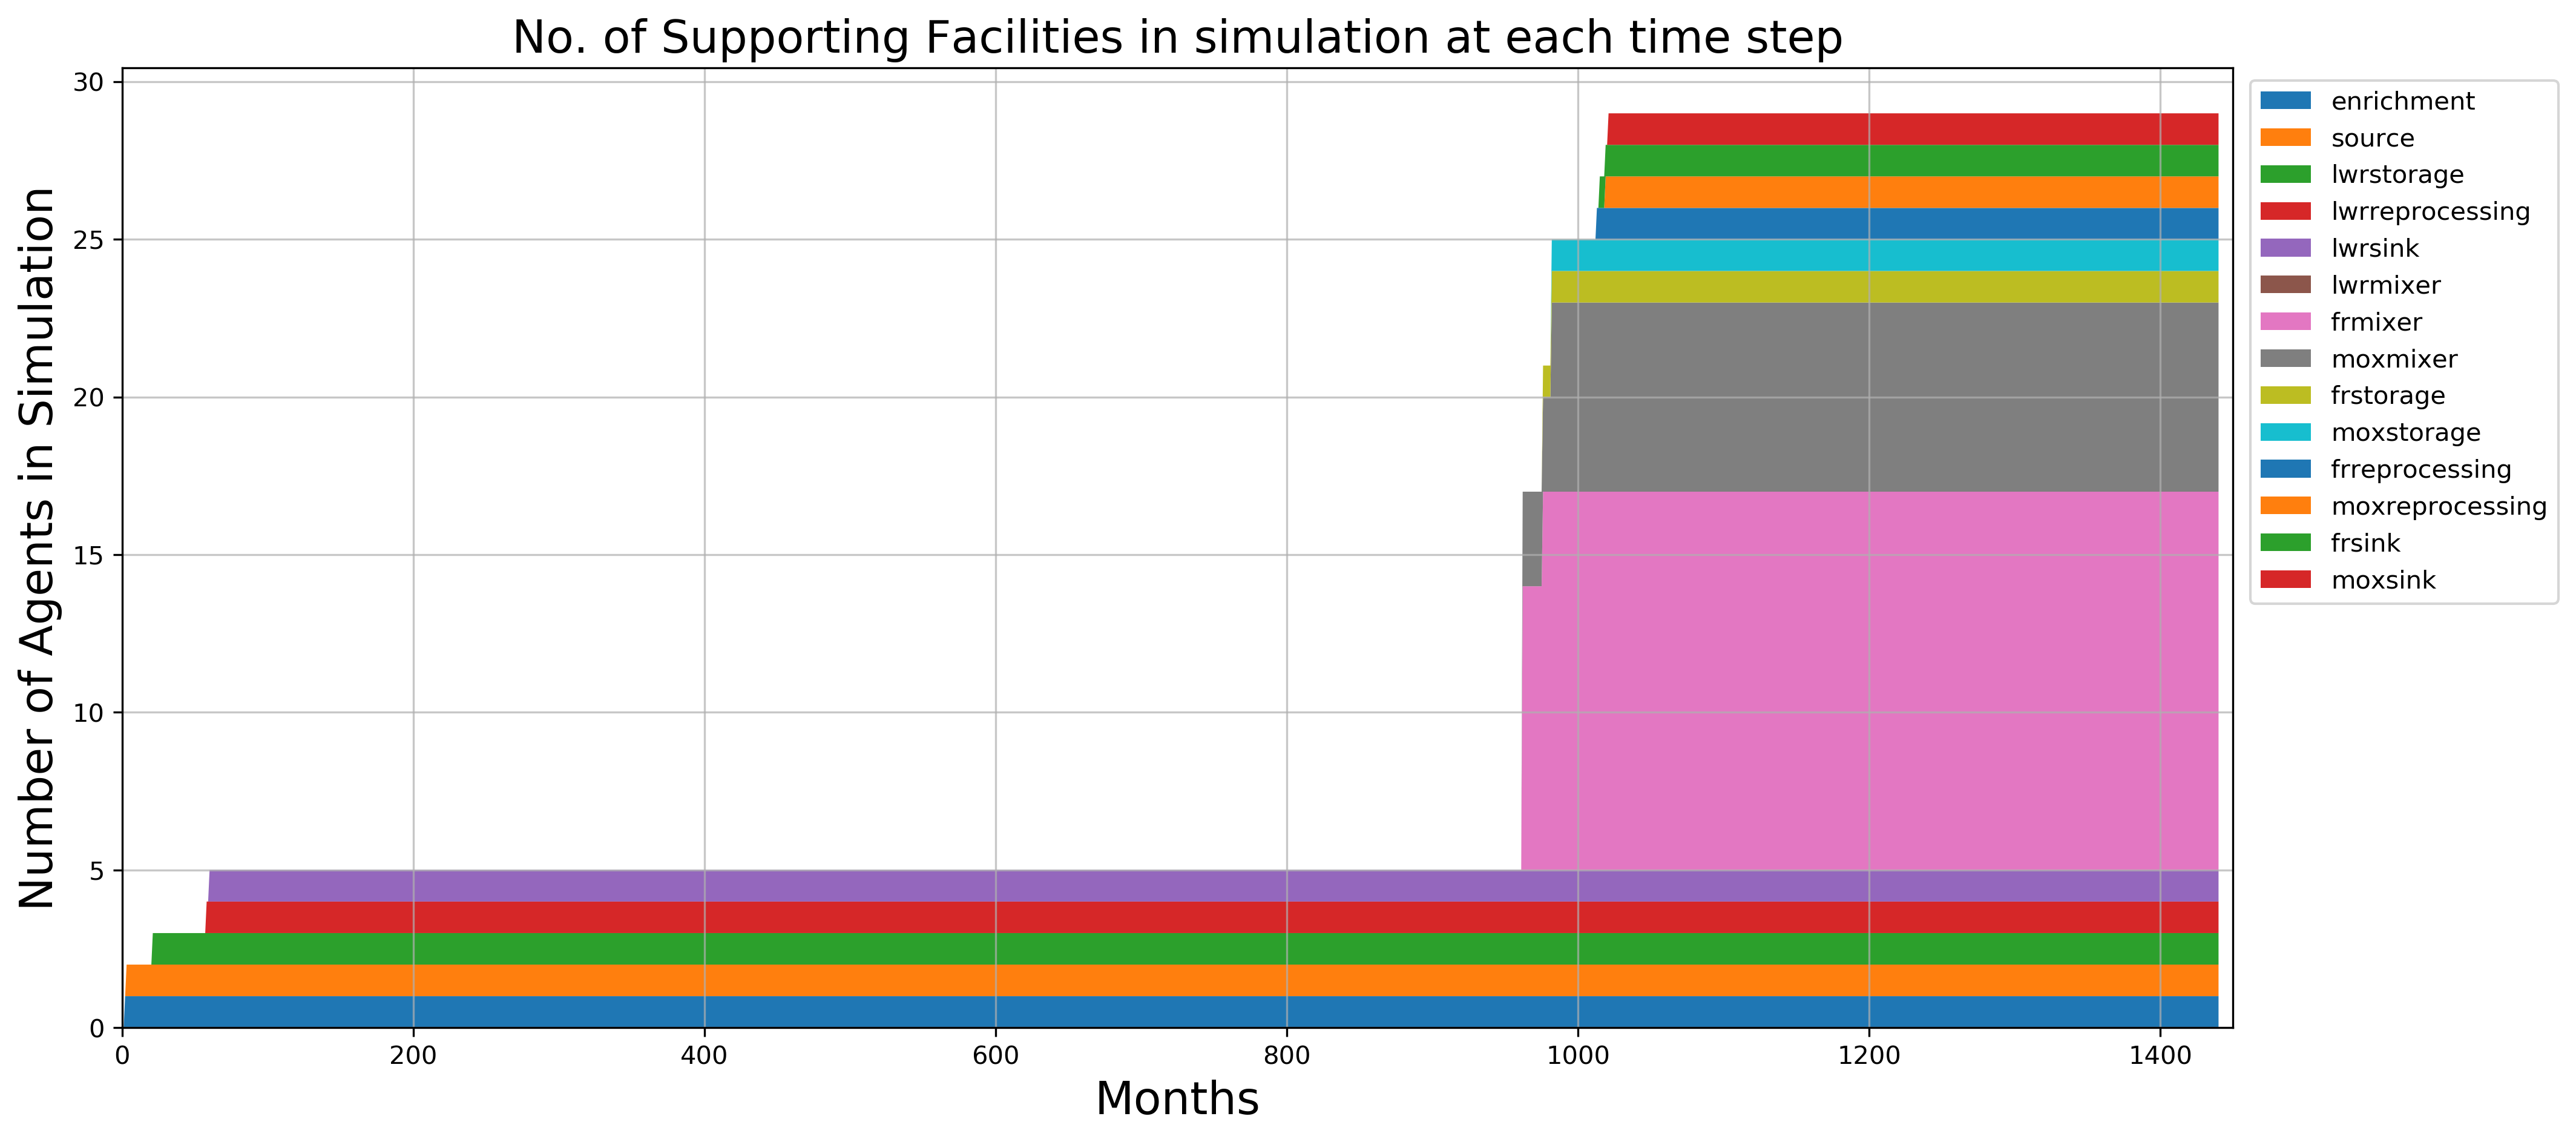
\includegraphics[width=\textwidth]{../paper/figures/eg30-stack_support.png}
        \end{center}
              \caption{Time dependent deployment of supporting facilities in 
              the EG01-30 linearly increasing power demand transition scenario. 
              \deploy automatically deploys reactor facilities 
              to set up a supply chain to meet constant power demand of $60000+250t/12$ MW
              during a transition from \glspl{LWR} to \glspl{SFR}. Note: \glspl{SFR}
              in this simulation have $\frac{1}{3}$ power capacity of \glspl{PWR}.}
      \end{figure}
\end{frame}

\begin{frame}
    \frametitle{Best Performing Transition Scenarios}
    \textbf{Undersupply and under capacity of commodities for the best performing transition scenarios} 
    \begin{table}[]
        \centering
            \caption{Undersupply/capacity of commodities for the best performing transition scenarios.}
            \label{tab:all-power}
            \footnotesize
            \begin{tabularx}{\textwidth}{l|RRRR}
            \hline
            & \multicolumn{3}{|c}{\textbf{Undersupplied Time Steps}} \\ \hline
            \textbf{Transition Scenario} & EG01-EG23 & 
            EG01-EG24 & EG01-EG29 & 
            EG01-EG30 \\ 
            \textbf{Power Demand} &Constant&Linearly Increasing&Constant&Linearly Increasing \\
            \textbf{Prediction Method} &\texttt{poly}&\texttt{fft}&\texttt{poly}& \texttt{fft}\\
            \textbf{Power Supply Buffer [MW]} &0&6000&0&8000 \\ \hline
            \textbf{Commodities} \\ 
            Natural Uranium		    & 2 	& 3  &  1  & 1 \\ 
            \gls{LWR} Fuel     	    & 4 	& 6  &  1  & 2\\ 
            \gls{SFR} Fuel     	    &  0 	& 0  &  2  & 2\\ 
            \gls{MOX} \gls{LWR} Fuel &-&-&2&2 \\
            Power      				&  6 	& 7  &  4 &  5\\ 
            \gls{LWR} Spent Fuel	& 1 	& 1  & 1 & 1\\ 
            \gls{SFR} Spent Fuel     	    &  1 	& 1  &  1  & 1\\ 
            \gls{MOX} \gls{LWR} Spent Fuel &-&-&1&1 \\ \hline 
        \end{tabularx}
    \end{table}
    
\end{frame}
\section{Conclusion}
\subsection{Conclusion}
\begin{frame}
  \frametitle{Conclusion}
        These results demonstrate that by carefully selecting \deploy 
        parameters, we are able to \textbf{effectively automate deployment}
        of reactors and supporting facilities to simulate
        constant and linearly increasing power demand transition scenarios
        for EG01-23, EG01-24, EG01-29, and EG01-30 with minimal 
        power undersupply. 
        \vspace{1em}
        \\
        Not completely eliminating undersupply and under capacity of 
        commodities in the simulation is expected 
        since without time series data 
        at the beginning of the simulation, \deploy takes a few 
        time steps to collect time series data about power demand 
        to predict and start deploying reactor and supporting 
        fuel cycle facilities. 
        
\end{frame}

\begin{frame}
  \frametitle{Future Work}
  \deploy can be used to conduct nuclear fuel cycle \textbf{sensitivity studies}. 
  One of the key issues facing nuclear fuel cycle transition scenario 
  simulations is the presence 
  of idle reactor capacity due to the lack of Pu to fabricate advanced fuels 
  in the simulation. 
  Previously, to conduct sensitivity analysis,  the user would have to manually 
  calculate the deployment scheme for every change in input parameter to avoid 
  idle capacity. 
\end{frame}
\subsection{Future Work}
%\input{future_work}
\begin{frame}
  \frametitle{Acknowledgement}
  This work is supported by U.S. Department of Energy, 
  Nuclear Energy University Program, under contract 
  \#NEUP-FY16-10512. 
  \end{frame}

%%--------------------------------%%
%%--------------------------------%%
\begin{frame}[allowframebreaks]
  \frametitle{References}
  \bibliographystyle{plain}
  {\footnotesize \bibliography{../paper/bibliography.bib} }

\end{frame}

%%--------------------------------%%


\end{document}



